\documentclass[12pt,a4paper]{report}

\usepackage{styles/dolgozat}

\usepackage{listings}
\usepackage{styles/cpp}
\usepackage{styles/python}

\usepackage{hyperref}

\usepackage{parskip}

\usepackage{tabularx}
\usepackage{ltablex}

\begin{document}

\pagestyle{empty} %a címlapon ne legyen semmi=empty, azaz nincs fejléc és lábléc

% A Miskolci Egyetem címere
{\large
\begin{center}
\vglue 1truecm
\textbf{\huge\textsc{Szakdolgozat}}\\
\vglue 1truecm

\includegraphics[width=4.8truecm, height=4truecm]{images/me_logo.png}\\
\textbf{\textsc{Miskolci Egyetem}}
\end{center}}

\vglue 1.5truecm %függõleges helykihagyás

% A szakdolgozat címe, akár több sorban is
{\LARGE
\begin{center}
\textbf{Tesztvezérelt programozás oktatás}
\end{center}}

\vspace*{2.5truecm}
% A hallgató neve, évfolyam, szak(ok), a konzulens(ek) neve
{\large
\begin{center}
\begin{tabular}{c}
\textbf{Készítette:}\\
Streba Dániel\\
Programtervező informatikus
\end{tabular}
\end{center}
\begin{center}
\begin{tabular}{c}
\textbf{Témavezető:}\\
Piller Imre
\end{tabular}
\end{center}}
\vfill
% Keltezés: Hely, év
{\large
\begin{center}
\textbf{\textsc{Miskolc, 2020}}
\end{center}}

\newpage


\newpage

\pagestyle{empty}

%Feladatkiiras
\begin{flushleft}
\textsc{\bfseries Miskolci Egyetem}\\
Gépészmérnöki és Informatikai Kar\\
Alkalmazott Matematikai Intézeti Tanszék\hspace*{4cm}\hfil \textbf{Szám:}
\end{flushleft}
\vskip 0.5cm
\begin{center}
\large\textsc{\bfseries Szakdolgozat Feladat}
\end{center}
\vskip 0.5cm
Streba Dániel (H0SRE6) programtervező informatikus jelölt részére.\newline

\noindent\textbf{A szakdolgozat tárgyköre:} szoftvertesztelés, webalkalmazás, oktatás\newline

\noindent\textbf{A szakdolgozat címe:} Tesztvezérelt programozás oktatás\newline

\noindent\textbf{A feladat részletezése:}

\medskip

\emph{
A tesztvezérelt fejlesztés (Test Driven Development) egy előnyös módszernek bizonyult a szoftverfejlesztés területén. A dolgozat a programozás oktatása esetében vizsgálja azt, hogy a tesztek készítésének, az azokkal történő számonkérésnek milyen előnyei, esetlegesen hátrányai lehetnek.
}

\medskip

\emph{
A dolgozat bemutatja egy webalkalmazás elkészítését, annak funkcióit, amelyben az elkészített tananyagokat el lehet helyezni, a diákok/hallgatók szerkeszthetik és ellenőrízhetik a feladatokhoz tartozó programkódokat. A program figyelmezteti a felhasználót a gyakran előforduló hibákkal kapcsolatban. A program a feladat elkészítését nyomonköveti, segítve ezzel az értékelést és a feladatok megoldási módjának vizsgálatát.
}

\medskip

\emph{
Az alkalmazás szerver oldali része ASP.NET keretrendszerben készül. A böngészőben futó kliens alkalmazás elkészítéséhez Angular JavaScript keretrendszer kerül felhasználásra. Ennek megfelelően a dolgozatban szereplő oktatási anyagok, kódpéldák szintén C\# és JavaScript nyelven készülnek.
}

\vfill

\noindent\textbf{Témavezető:} Piller Imre (egyetemi tanársegéd) \newline

% \noindent\textbf{Konzulens(ek):} (akkor kötelezõ, ha a témavezetõ nem valamelyik matematikai tanszékrõl való; de persze lehet egyébként is)\newline

\noindent\textbf{A feladat kiadásának ideje:} 2020. szeptember 28.\newline

%\noindent\textbf{A feladat beadásának határideje:}

\vskip 2cm

\hbox to \hsize{\hfil{\hbox to 6cm {\dotfill}\hbox to 1cm{}}}

\hbox to \hsize{\hfil\hbox to 3cm {szakfelelős}\hbox to 2cm{}}

\newpage

\vspace*{1cm}  
\begin{center}
\large\textsc{\bfseries Eredetiségi Nyilatkozat}
\end{center}
\vspace*{2cm}  

Alulírott \textbf{Streba Dániel}; Neptun-kód: \texttt{H0SRE6} a Miskolci Egyetem Gépészmérnöki és Informatikai Karának végzős Programtervező informatikus szakos hallgatója ezennel büntetőjogi és fegyelmi felelősségem tudatában nyilatkozom és aláírásommal igazolom, hogy \textit{Tesztvezérelt programozás oktatás}
című szakdolgozatom saját, önálló munkám; az abban hivatkozott szakirodalom
felhasználása a forráskezelés szabályai szerint történt.\\

Tudomásul veszem, hogy szakdolgozat esetén plágiumnak számít:
\begin{itemize}
\item szószerinti idézet közlése idézőjel és hivatkozás megjelölése nélkül;
\item tartalmi idézet hivatkozás megjelölése nélkül;
\item más publikált gondolatainak saját gondolatként való feltüntetése.
\end{itemize}

Alulírott kijelentem, hogy a plágium fogalmát megismertem, és tudomásul veszem, hogy
plágium esetén szakdolgozatom visszautasításra kerül.

\vspace*{3cm}

\noindent Miskolc, \hbox to 2cm{\dotfill} .év \hbox to 2cm{\dotfill} .hó \hbox to 2cm{\dotfill} .nap

\vspace*{3cm}

\hspace*{8cm}\begin{tabular}{c}
\hbox to 6cm{\dotfill}\\
Hallgató
\end{tabular}



\newpage

\noindent 1.

\begin{tabular}{cl}
&szükséges (módosítás külön lapon) \\
A szakdolgozat feladat módosítása& \\
& nem szükséges\\
&\\
\hbox to 4cm{\dotfill}&\multicolumn{1}{c}{\hbox to 5cm{\dotfill}}\\
dátum& \multicolumn{1}{c}{témavezető(k)}
\end{tabular}
\vskip1.5mm

\noindent 2. A feladat kidolgozását ellenőriztem:

\vskip1.5mm

\begin{tabular}{l@{\hspace*{4cm}}l}
témavezető (dátum, aláírás):& konzulens (dátum, aláírás):\\
\dotfill&\dotfill\\
\dotfill&\dotfill\\
\dotfill&\dotfill
\end{tabular}

\vskip1.5mm

\noindent 3. A szakdolgozat beadható:

\vskip1.5mm

\begin{tabular}{@{\hspace*{1.3cm}}c@{\hspace*{2.1cm}}c}
\hbox to 4cm{\dotfill}&\multicolumn{1}{c}{\hbox to 5cm{\dotfill}}\\
dátum& \multicolumn{1}{c}{témavezető(k)}
\end{tabular}

\vskip1.5mm

\noindent 4.
\begin{tabular}[t]{@{}l@{\hspace*{1mm}}l@{\hspace*{1mm}}l@{}}
A szakdolgozat& \hbox to 3.5cm{\dotfill} &szövegoldalt\\
              & \hbox to 3.5cm{\dotfill} &program protokollt (listát, felhasználói leírást)\\
              &\hbox to 3.5cm{\dotfill}   &elektronikus adathordozót (részletezve)\\
              &\hbox to 3.5cm{\dotfill} & \\
              &\hbox to 3.5cm{\dotfill} &egyéb mellékletet (részletezve)\\
              &\hbox to 3.5cm{\dotfill} &\\
\end{tabular}
\newline tartalmaz.

\vskip1.5mm

\begin{tabular}{@{\hspace*{1.3cm}}c@{\hspace*{2.1cm}}c}
\hbox to 4cm{\dotfill}&\multicolumn{1}{c}{\hbox to 5cm{\dotfill}}\\
dátum& \multicolumn{1}{c}{témavezető(k)}
\end{tabular}

\noindent 5.

\begin{tabular}{ll}
&bocsátható\\
A szakdolgozat bírálatra& \\
& nem bocsátható\\
\end{tabular}

\vskip1.5mm

\noindent A bíráló neve: \hbox to 8cm{\dotfill}

\vskip4mm

\begin{tabular}{@{\hspace*{1.3cm}}c@{\hspace*{2.1cm}}c}
\hbox to 4cm{\dotfill}&\multicolumn{1}{c}{\hbox to 5cm{\dotfill}}\\
dátum& \multicolumn{1}{c}{szakfelelős}
\end{tabular}

\noindent 6.
\begin{tabular}[t]{@{}l@{\hspace*{1mm}}l@{\hspace*{1mm}}l@{}}
A szakdolgozat osztályzata& &\\
&a témavezető javaslata:& \hbox to 3cm{\dotfill}\\
&a bíráló javaslata:& \hbox to 3cm{\dotfill}\\
&a szakdolgozat végleges eredménye:& \hbox to 3cm{\dotfill}
\end{tabular}

\vspace*{4mm}

\noindent Miskolc, \hbox to 4.5cm{\dotfill} \hspace*{2.5cm}
\begin{tabular}[t]{cc}
\hbox to 6cm{\dotfill}\\
a Záróvizsga Bizottság Elnöke
\end{tabular}


\cleardoublepage
\pagenumbering{gobble}
\tableofcontents
\cleardoublepage
\pagenumbering{arabic}

\newpage

\pagestyle{fancy}

\Chapter{Bevezetés}

A fejezet célja, hogy a feladatkiírásnál kicsit részletesebben bemutassa, hogy miről fog szólni a dolgozat.
Érdemes azt részletezni benne, hogy milyen aktuális, érdekes és nehéz probléma megoldására vállalkozik a dolgozat.

Ez egy egy-két oldalas leírás.
Nem kellenek bele külön szakaszok (section-ök).
Az irodalmi háttérbe, a probléma részleteibe csak a következő fejezetben kell belemenni.
Itt az olvasó kedvét kell meghozni a dolgozat többi részéhez.

\Chapter{Koncepció}

% Ez a fejezet még nem a saját eredményekkel foglalkozik, hanem bemutatja, mi a problémakör, milyen módszerekkel, milyen eredményeket sikerült elérni eddig másoknak.

% A hivatkozások jelentős része ehhez a fejezethez szokott kötődni.
% (Egy hivatkozás például így néz ki \cite{coombs1987markup}.)
% Itt lehet bemutatni a hasonló alkalmazásokat.

% A fejezet tartalma témától függően változhat. Az alábbiakat attól függően különböző arányban tartalmazhatják.

% % Amit csak említés szintjén érdemes szerepeltetni

% Az olvasóról annyit feltételezhetünk, hogy programozásban valamilyen szinten járatos, és a matematikai alapfogalmakkal sem ebben a dolgozatban kell megismertetni.
% A speciális eszközök, programozási nyelvek, matematikai módszerek és jelölések persze jó, hogy ha említésre kerülnek, de nem kell nagyon belemenni a közismertnek tekinthető dolgokba.

\Section{Irodalomkutatás}

% Amennyiben a dolgozat egy módszer kidolgozására, kifejlesztésére irányul, akkor itt lehet részletesen végignézni (módszertani vagy időrendi bontásban), hogy az eddigiekben milyen eredmények születtek a témakörben.

\SubSection{Egységtesztelés}

Az egységtesztelés (\emph{unit testing}) a szoftvertesztelés egy olyan módszere, amely során a forráskód legalacsonyabb szintű, a programot felépítő egységeket tesztelik. A szoftvertesztelés szintjei \aref{fig:software_testing_levels}. ábrán látható. Az egység egy rendszer legkisebb önálló egységként tesztelhető része. Az egységtesztekkel ellenőrizhető, hogy egy egység az elvárásoknak megfelelően működik. Egy egység függvényeiről ellenőrizzük, hogy különböző bemenetek esetén megfelelő eredményt, vagy hibát produkálnak. Az egységeket egymástól függetlenítve kell tesztelni.

\begin{figure}[h]
    \centering
    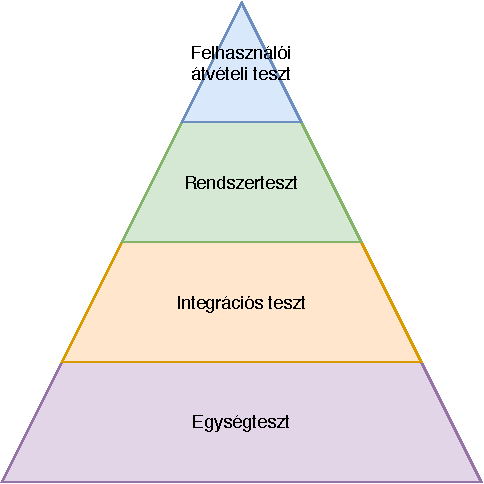
\includegraphics{images/software_testing_levels.pdf}
    \caption{A szoftvertesztelés szintjei.}
    \label{fig:software_testing_levels}
\end{figure}

Az egységtesztelés nem egy új fogalom a szoftverfejlesztésben. Az 1970-es évektől, a Smalltalk programozási nyelv korai napjai óta jelen van, és ez az egyik legjobb módszer arra, hogy a fejlesztő növelje a kód minőségét miközben jobban megérti az adott osztály vagy metódus működését. Kent Beck amerikai szoftvermérnök vezette be az egységtesztelés koncepcióját, majd ezután az egységtesztelés, mint fogalom átöröklődött sok más programozási nyelvbe is, ezzel az egységtesztelést egy rendkívül hasznos, és nyelvfüggetlen gyakorlattá téve. \cite{osherove_2013_the-art-of-unit-testing}

Beck az egységtesztelést a Smalltalk nevű programozási nyelvben implementálta az SUnit egységtesztelő keretrendszerként. \cite{beck_1999_guide-to-better-smalltalk} Ezután a keretrendszert a fejlesztői közösség adaptálta más programozási nyelvekre is és megtartották a Beck által bevezetett terveket, ötleteket. Az SUnit-ot alapul vevő egységtesztelő keretrendszereket nevezzük összefoglaló néven xUnit keretrendszereknek. \cite{fowler_2006_xunit}

Napjainkban a legnépszerűbb egységteszt keretrendszerek mind az xUnit keretrendszercsaládba tartoznak.

\SubSection{Tesztvezérelt fejlesztés}

A tesztvezérelt fejlesztés (\emph{Test-driven Development}, \emph{TDD}) napjaink egyik legismertebb szoftverfejlesztési folyamata a professzionális programozásban. Ez a folyamat nagyon rövid fejlesztési ciklusokon alapul: a követelmények nagyon specifikus tesztesetekként vannak megfogalmazva, a kódot pedig ahhoz mérten írjuk, hogy az át fog így menni a teszten. Ez teljes ellentettje a hagyományos szoftverfejlesztésnek, mivel az megengedi azon kódrészleteket is, amelyek nem felelnek meg a követelményeknek teljesen.

Az egységteszteléshez hasonlóan ez is Kent Beck-től ered. Őt tartjuk számon a technika kifejlesztéséért, és újrafelfedezésért. Beck a tesztvezérelt fejlesztésről először egy régi programozásról szóló könyvben olvasott, majd amikor megírta az első xUnit keretrendszert a Smalltalk nyelvben, akkor emlékezett erre, majd kipróbálta ezt saját maga is. \cite{beck_2012_tdd-rediscovery} A tesztvezérelt fejlesztés folyamatát az extrém programozás (\emph{Extreme Programming}) nevű módszertan részeként tökéletesítette és ekkor vált népszerűvé ez a módszer a programozók körében.

\begin{figure}[h]
    \centering
    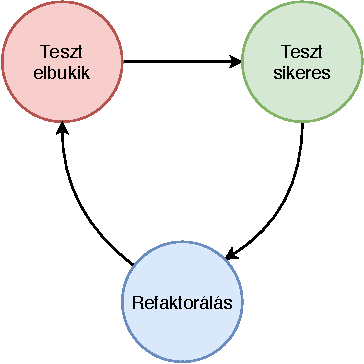
\includegraphics{images/tdd_steps.pdf}
    \caption{A tesztvezérelt fejlesztés ciklusa és azon lépései.}
    \label{fig:tdd_steps}
\end{figure}

A tesztvezérelt fejlesztés ciklusának \aref{fig:tdd_steps} ábrán látható lépései kifejtve: \cite{beck_2003_tdd}
\begin{enumerate}
    \item \textbf{Tesztírás}

          Minden új funkció fejlesztése tesztek írásával kezdődik. Minden frissíteni kívánt vagy újdonsült metódushoz írjunk egy tesztet ami röviden és tömören lefedi az új funkciót. Ehhez a fejlesztőnek tisztán értenie kell a funkció specifikációját és követelményeit. A fejlesztő ezt használati eset (\emph{use case}) diagramokon vagy felhasználói történeteken (\emph{user story}) keresztül értheti meg a követelményeket, majd ezek után foghat neki megírni a teszteseteket. Ezek lehetnek már meglévő tesztesetek bővítései is, ha egy meglévő funkciót bővít ki.

    \item \textbf{Tesztfuttatás}

          A tesztesetek megírása után mindenképpen érdemes lefuttatni azokat, mivel jelen állapotban minden tesztesetnek el kell buknia. Ilyenkor még nincs az új funkcióhoz tartozó programkód megírva, és az ilyenkor elbukott tesztesetek garantálják azt, hogy nem írt a programozó olyan tesztet ami mindig sikeres, ami hibás lenne.

    \item \textbf{Kódírás}

          Ebben a lépésben a fejlesztő megírja a tesztesetekhez tartozó működő programkódot. Fontos, hogy az itt megírt programkódnak nem kell tökéletesnek lennie, itt az a cél, hogy mindegyik teszteset sikeresen lefusson. A programozónak nem szabad a teszteseteket meghaladó, a specifikáción és követelményeken kívül eső kódot írnia.

    \item \textbf{Tesztfuttatás}

          Ha az összes teszteset sikeresen lefut, akkor a programozó biztos lehet benne, hogy az új kód megfelel a teszt specifikációknak és nem tör el vagy ront el más funkciókat. Ha a tesztesetek közül legalább 1 darab nem fut le, akkor a kódot addig kell javítanunk míg az összes teszteset sikeres nem lesz.

    \item \textbf{Refaktorálás}

          A növekvő kódbázist folyamatosan takarítani kell a tesztvezérelt fejlesztés során. Az új kód átmozgatásra kerülhet a logikailag, és strukturálisan megfelelő helyére. A kódduplikációkat ki kell szervezni, el kell távolítani. A osztályaink, változóink és metódusaink elnevezését javítani kell, hogy mások is tisztán érthessék a funkciókat. Ahogy új és új funkciók hozzáadásra kerülnek az osztályaink és a metódusaink egyre és egyre hosszabbak lesznek, ezeket gondosan szét kell darabolni több részre az olvashatóság és karbantarthatóság miatt.

          A tesztesetek folyamatos futtatása segíti abban a fejlesztőt, hogy a refaktorálás lépése alatt elvégzett kód átírások során nem tör el semmi funkciót és a tesztek ugyanúgy sikeresen lefutnak.
\end{enumerate}

\SubSection{Egységtesztelés a C\# programozási nyelvben}

A C\# programozási nyelvben nincs gyári, beépített (azaz a .NET keretrendszerrel érkező) egységtesztelő keretrendszer, így mind a tesztek írásához, futtatásához és az eredmények megjelenítéséhez szükségünk van egy ezt támogató bővítményre.

Napjainkban a legnépszerűbb egységteszt keretrendszerek a következők:
\begin{itemize}
    \item[--] Visual Studio Unit Testing Framework azaz MSTest
    \item[--] xUnit.net
    \item[--] NUnit
\end{itemize}

Mindhárom keretrendszer ingyenes, és nyílt forráskódú. Az MSTest keretrendszert habár a Microsoft fejleszti, szintén mint a C\# nyelvet és a .NET környezetet, de ez nincs a környezetbe integrálva. Az xUnit.net-et a Microsoft hivatalosan is használja több szoftverének tesztelésében is, például az ASP.NET Core forráskódhoz ezzel a keretrendszerrel készítik az egységteszteket.

A szakdolgozatban keretében a xUnit.net keretrendszer kerül felhasználásra.

Ezeket a keretrendszereket többféleképpen is elérhetjük a programunkban.
Legegyszerűbb módja ennek a keretrendszer bináris csomagjának a NuGet csomagkezelő rendszeren való letöltése, de ezenkívül a nyílt forráskódú csomagokat mi is lefordíthatjuk és manuálisan behivatkozhatjuk a projektfájlunkban, vagy akár a keretrendszer honlapjáról is letölthetjük a már lefordított binárisokat.

Miután telepítettük az általunk választott keretrendszert, elkezdhetünk írni egységteszteket a kódunkhoz. Minden megfelelően annotált metódus egy teszteset amiben egy másik adott kódot tesztelünk. Minden keretrendszernél kicsit másképpen néz ki a tesztek felépítése, de bevett szokás az, hogy az teszteseteket tartalmazó metódusokat annotálnunk kell. xUnit.net esetén a metódust a \texttt{Fact} ("mindig igaz" teszteset) vagy \texttt{Theory} ("a megfelelő adatra igaz" teszteset) attribútummal kell annotálnunk, ezzel jelezzük a keretrendszerünknek, hogy az adott metódus egy teszteset.

Nagyobb kódbázis esetén átláthatatlan ha minden tesztesetet a tesztelendő osztályba raknánk bele ezért más keretrendszereknél elvárt az, hogy az egységteszteink számára új osztályt hozzunk létre. Bevett szokás az, hogy új projektet hozunk létre ahol csak a tesztek osztályait és azok segítő osztályait tároljuk, de az is elegendő ha a meglévő projektben hozzuk létre az egységteszt osztályainkat. Az osztály létrehozása után, metódusonként írhatjuk meg a teszteseteinket. Az xUnit.net-nél erre nincs szükség, azonban javasolt, hogy elkülönítve és jól megnevezve tároljuk a teszteseteket tartalmazó osztályokat és magukat a metódusokat.

Minden keretrendszerben elérhető egy \texttt{Assert} osztály, amivel állításokat tehetünk a tesztjeinkbe. Ellenőrizhetjük, hogy például a metódusunk visszatérési értéke azaz az tényleges (\emph{actual}) érték megegyezik-e a várt (\emph{expected}) értékkel. Ezenkívül szinte bármilyen más feltételt ellenőrizhetünk. Például, hogy a tényleges érték tartalmaz-e valamit, üres-e, a várt típusú-e vagy, hogy éppen dob-e kivételt vagy sem. A teszteset akkor kerül sikeres (\emph{pass}) állapotba, ha minden állításnak megfelelt, és közben nem dobott-e a programunk le nem kezelt kivételt. Ha ezeket nem teljesíti a tesztesetünk akkor sikertelen (\emph{fail}) állapotba kerül.

\Section{Piackutatás}

% Bizonyos témáknál új termék vagy szolgáltatás kifejlesztése a cél.
% Ekkor érdemes annak alaposan utánanézni, hogy aktuálisan milyen eszközök érhetők el a piacon.
% Ez szoftverek esetében a hasonló alkalmazások bemutatását, táblázatos formában történő összehasonlítását jelentheti.
% Szerepelhetnek képek és észrevételek a viszonyításként bemutatott alkalmazásokhoz.

Ebben az alfejezetben a szakdolgozat témájához kapcsolódó, aktuálisan elérhető hasonló szoftverek és alkalmazások kerülnek bemutatásra.

Napjainkban nagyon elterjedt lett a tesztvezérelt fejlesztés, és a tesztvezérelt oktatás pedig ebből a módszerből fejlődött ki. Ez egy rendkívül felkapott témakör, több cég építette már ki erre a teljes portfólióját, és rengeteg weboldal, alkalmazás készült már ami a manuális, emberi erőforrásokon alapuló programozás oktatást szeretné leváltani, megkönnyíteni azáltal, hogy egy teljesen automatizáltan működő tanulóprogramot ad a programozást tanulni kívánók kezébe.

\SubSection{Mester}

A Mester egy ingyenesen használható online programozási feladatbank. Ez az Eötvös Lóránd Tudományos Egyetem Informatikai Karának egyik rendszere. \cite{elte-mester} A Mester mindenki számára elérhető egy ingyenes regisztráció után, viszont létezik egy Biró nevű változata, amit csak a karon tanuló hallgatók érhetnek el zárthelyi dolgozatok és beadandó feladatok megírásához. \cite{elte-biro}

\begin{figure}[h]
    \centering
    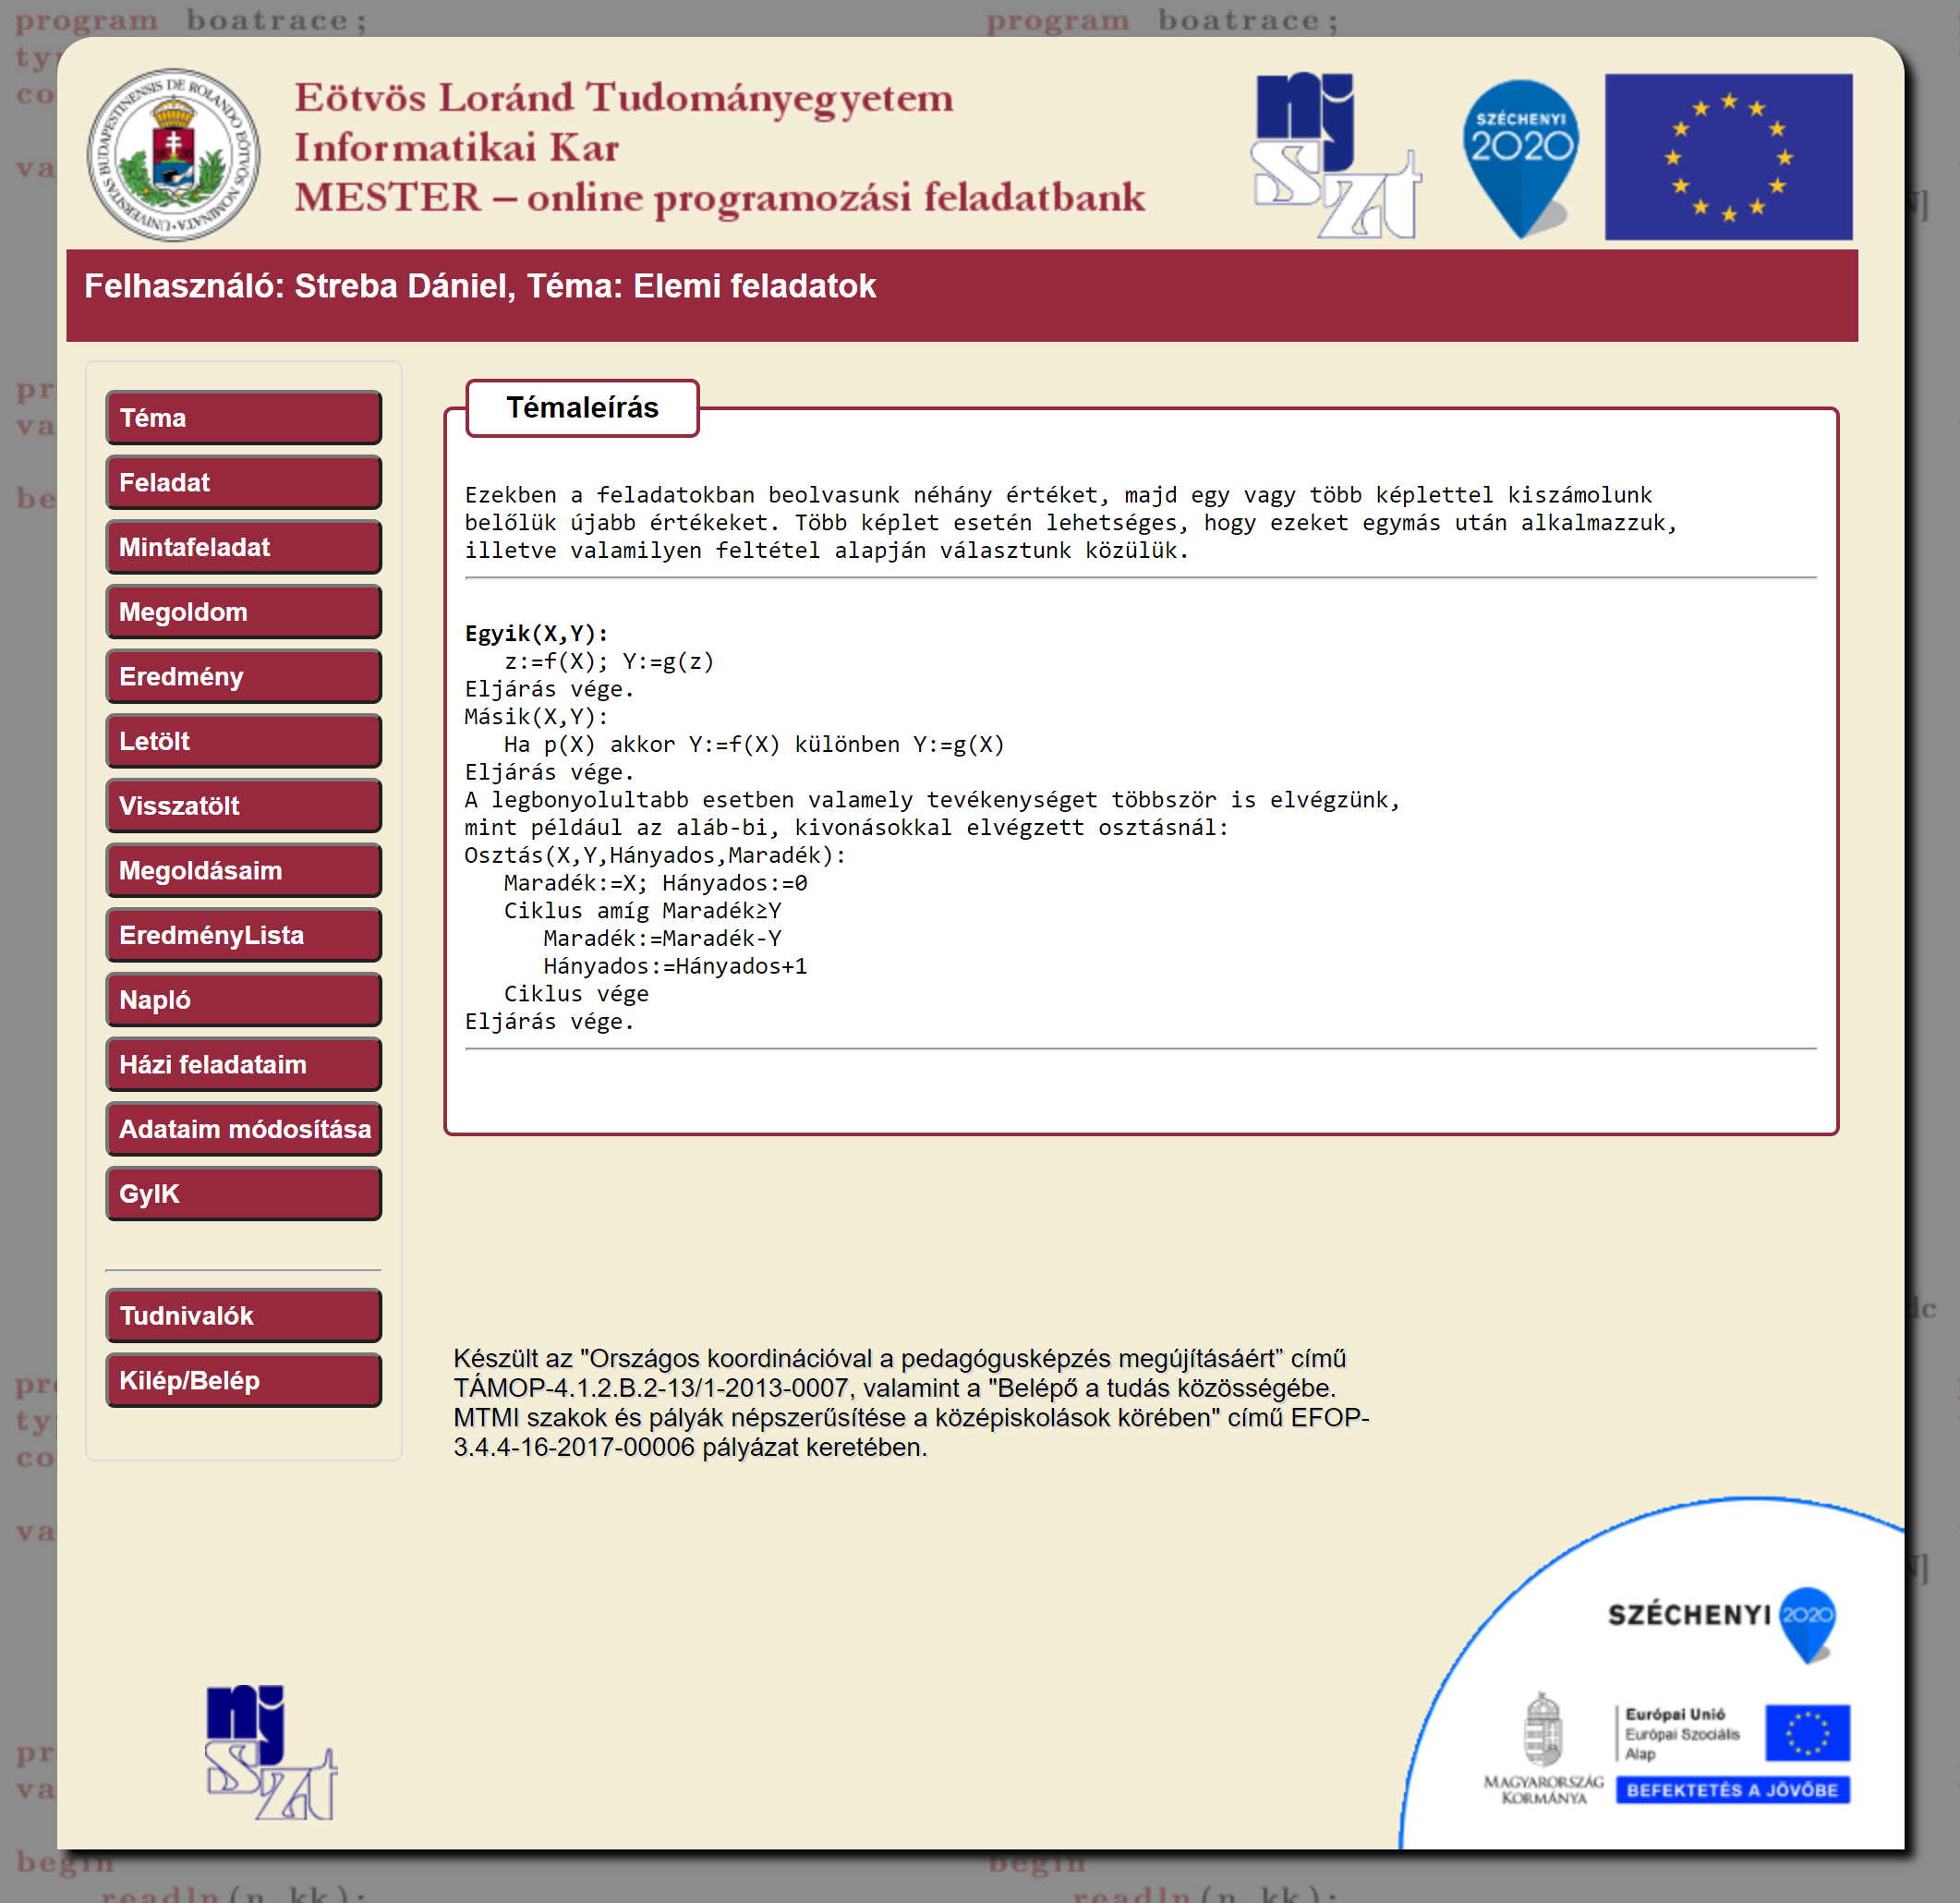
\includegraphics[width=0.95\textwidth]{images/mester.png}
    \caption{Az Mester főoldala.}
    \label{fig:mester}
\end{figure}

A Mesteren rengeteg programozási feladat található, mind magyarul és mind bekategorizálva.

A feladatokat a következőképpen érhetjük el:
\begin{enumerate}
    \item Szintválasztás

          Itt választhatunk kezdő, középhaladó illetve haladó szint közül. Ezenkívül még elérhető két versenyre felkészítő szint is: OKTV és diákolimpia.

    \item Témaválasztás

          A kezdő szinten belül például a programozási tételek vannak felbontva témákra.

          Középhaladó szinten érettségi feladatokat és egyedi tematizált feladat témaköröket (például: időjárás, verseny) találunk.

          Haladó szinten pedig rekurzióval foglalkozó, különféle algoritmusokkal, gráfokkal foglalkozó témaköröket találunk.

          Minden témához tartozik egy kidolgozott mintafeladat pszeudokódos, C++ illetve Pascal nyelven elérhető megoldással. Illetve a témakiválasztását követően találunk a főoldalon egy témaleírást amihez egy példa \aref{fig:mester} ábrán tekinthető meg.

    \item Feladatválasztás

          Itt magát a témán belüli feladatot választhatjuk ki.
\end{enumerate}

Kiválasztás után a feladatunkat PDF formátumban kapjuk meg, ebben megtaláljuk a feladatleírást, szöveges leírást arról, hogy milyen bemenetet és kimenetet vár el a feladatellenőrző, illetve ezekre kapunk 2-2 példát is. Ezenkívül a lap alján megtaláljuk a programunk futására megengedett időlimitet és a memórialimitet, amikhez optimalizálnunk kell a megoldásunkat.

Miután elkészítettük a megoldásunkat, azt feltölthetjük a weboldalra és a Mester feladatellenőrző modulja ellenőrzi azt. A modul képes ellenőrizni a programunk helyességét, illetve lefordítja és különféle bemenetekkel érkezett kimeneteket összehasonlít a letárolt megoldásokkal.

A Mester jelenleg 6 programozási nyelvet támogat. Ezek a következők: \cite{elte-mester_tudnivalok}
\begin{itemize}
    \item C és C++ (gcc 5.4.0)
    \item C\# és Visual Basic (mono 4.6.2)
    \item Java (jdk 1.8)
    \item Pascal (FreePascal 3.0.0)
    \item Python (cython 3.5)
\end{itemize}

Egy kisebb korlátozás a weboldalban, hogy programunkat az adott feladathoz csak limitált számmal tölthetjük fel, ezt a feladat készítője határozza meg. A legtöbb feladat esetében 20 próbálkozásunk áll rendelkezésünkre. Ez ösztönzi a tanulót arra, hogy a saját számítógépén próbálja meg a minta be- és kimenettel a programját, és csak akkor töltse fel, ha már azokra jól működik.

A tesztelés filozófiáját a Mester Gyakran ismételt kérdéseik aloldala a következőképpen fogalmazza meg:
\begin{quotation}
    \textsl{,,A feltöltött (tesztelendő) programot első lépésben lefordítja a megjelölt nyelv fordítóprogramjával. Ha a fordítás sikertelen, akkor vége. Második lépésben egy védett környezetben (figyelve az erőforrás korlátokat; memória és CPU idő) előre elkészített bemenetekre futtatja. Ha időlimiten belül szabályosan (0 kilépési kóddal) fejeződik be a futtatás, akkor a kapott kimenet helyességét ellenőrzi.''} \cite{elte-mester_gyik}
\end{quotation}
A megoldásunk pontozása egy 0-tól 100-ig terjedő skálán történik. A feladatok pontozását a feladat készítője határozza meg, ezt a feladatleírásban olvashatjuk el.

A weboldalon láthatjuk még az előző feladataink pontjait, a feladatellenőrző modul üzenetét és a futási időt is. Ugyanitt letölthetjük az előző megoldásaink kódját is.

A programunkban csak a standard függvénykönyvtárak használhatóak, és a platformspecifikus könyvtárak le vannak tiltva (ilyen például a Windows grafikus könyvtár). A programba értékek betöltése a standard bemenetről való beolvasással történik, és az eredmények kiíratása pedig a standard kimenetre való írásával. Ez azt jelenti, hogy a Mester nem használja a tesztvezérelt fejlesztéshez javasolt egységtesztelő könyvtárakat.

\SubSection{CodeWars}

A CodeWars egy gamifikált programozást oktató weboldal, ahol több mint 50 programozási nyelvből választhatunk a több mint 9000 feladat megoldásához. \cite{codewars}

\begin{figure}[h]
    \centering
    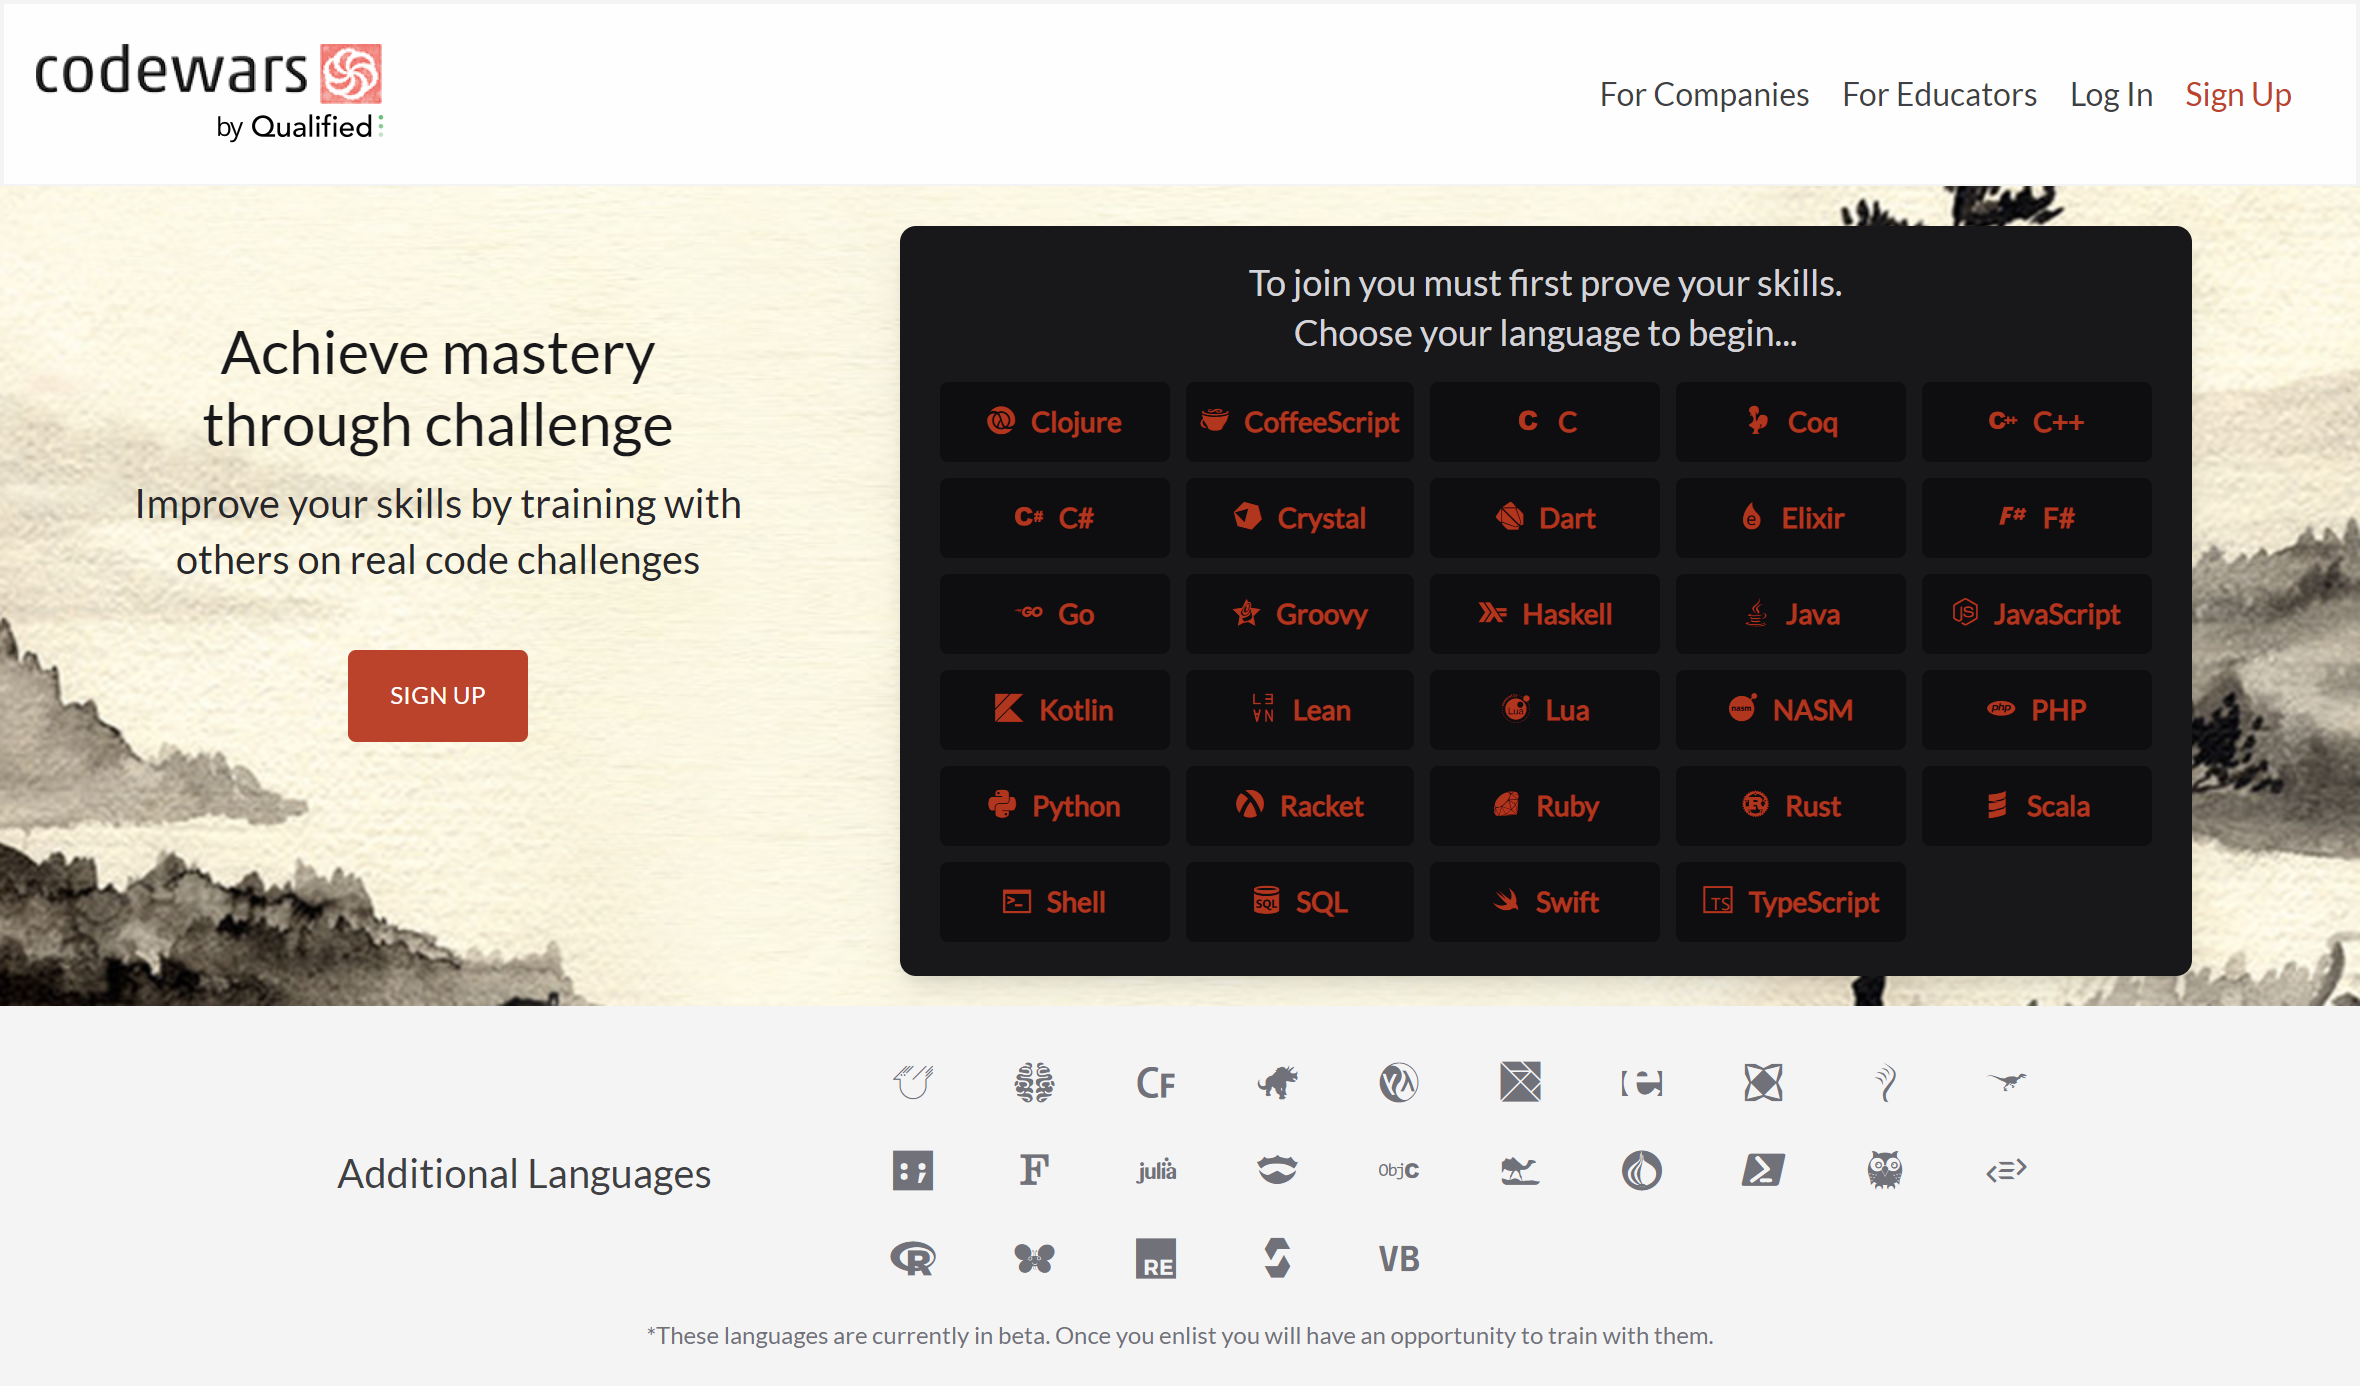
\includegraphics[width=0.95\textwidth]{images/codewars_homepage.png}
    \caption{A CodeWars főoldala.}
    \label{fig:codewars_homepage}
\end{figure}

A legnépszerűbb nyelvek mind támogatottak, mint például a C\#, Java, JavaScript, Python, de ezenkívül akár Fortran-ban vagy CommonLisp-ben is oldhatunk meg feladatokat. \Aref{fig:codewars_homepage} ábrán látható programozási nyelvek közül válogathatunk.

Az alkalmazást a Qualified nevű amerikai cég fejleszti, és a Qualified név alatt cégek interjúztatási procedúrájához is forgalmazzák a CodeWars professzionálisabbra szabott verzióját. \cite{qualified}

A CodeWars teljesen gamifikált rendszer, a játék részeként egy japán stílusú felületet alakítottak ki. A rendszerben a programozási feladatokat "kata"-nak hívják. A feladatok teljesítésért, esetleges hibák javításáért és minőségi megoldások feltöltésért pedig úgy nevezett "dicsőség" (\emph{honor}) pontokat és a pontok gyűjtésével rangokat kaphatunk. Más tanulók profiljait követhetjük és ők is követhetnek minket, és egymás profiljain láthatjuk az adott tanuló statisztikáit.

Több mint 9000 feladat közül válogathatunk, ezek nehézség és témakör címkék szerint vannak rendezve. A nehézséget a rendszer 1-től 8 "kyu"-ig méri, a legkönnyebb feladatok a 8 "kyu" kategóriába tartoznak, és az 1 "kyu"-ig nehezednek.

A feladatokat megnyitva láthatjuk a Markdown formátumban készített feladatleírást, amiben sokszor \LaTeX{} képletekkel van levezetve a matematikai rész, illetve látjuk a feladat címkéit, azt hogy, kik készítették a feladatot, és ha már 1 programozási nyelven megoldottuk akkor látjuk az ahhoz tartozó megoldásokat más tanulóktól, illetve a teszteseteket ami alapján tesztelte a rendszer a megoldásunkat.
A megoldásokhoz hozzászólhatunk és értékelhetjük is. Ugyanezt szintén megtehetjük magával a feladattal is.

Az alkalmazás a tesztvezérelt oktatás elvét követi, és a Mesterrel ellentéttel ez már egységtesztelő keretrendszereket használ a megoldásaink ellenőrzésére. Itt nem a standard be- és kimenet van használva, hanem a feladat megnyitásakor kapunk egy előredefiniált osztály- és metódusvázt amiben meg van adva nekünk, hogy milyen paraméterekkel lesz meghívva a metódusunk (ez a bemenet), és milyen visszatérési értéket vár (ez lesz a kimenet).

\begin{figure}[h]
    \centering
    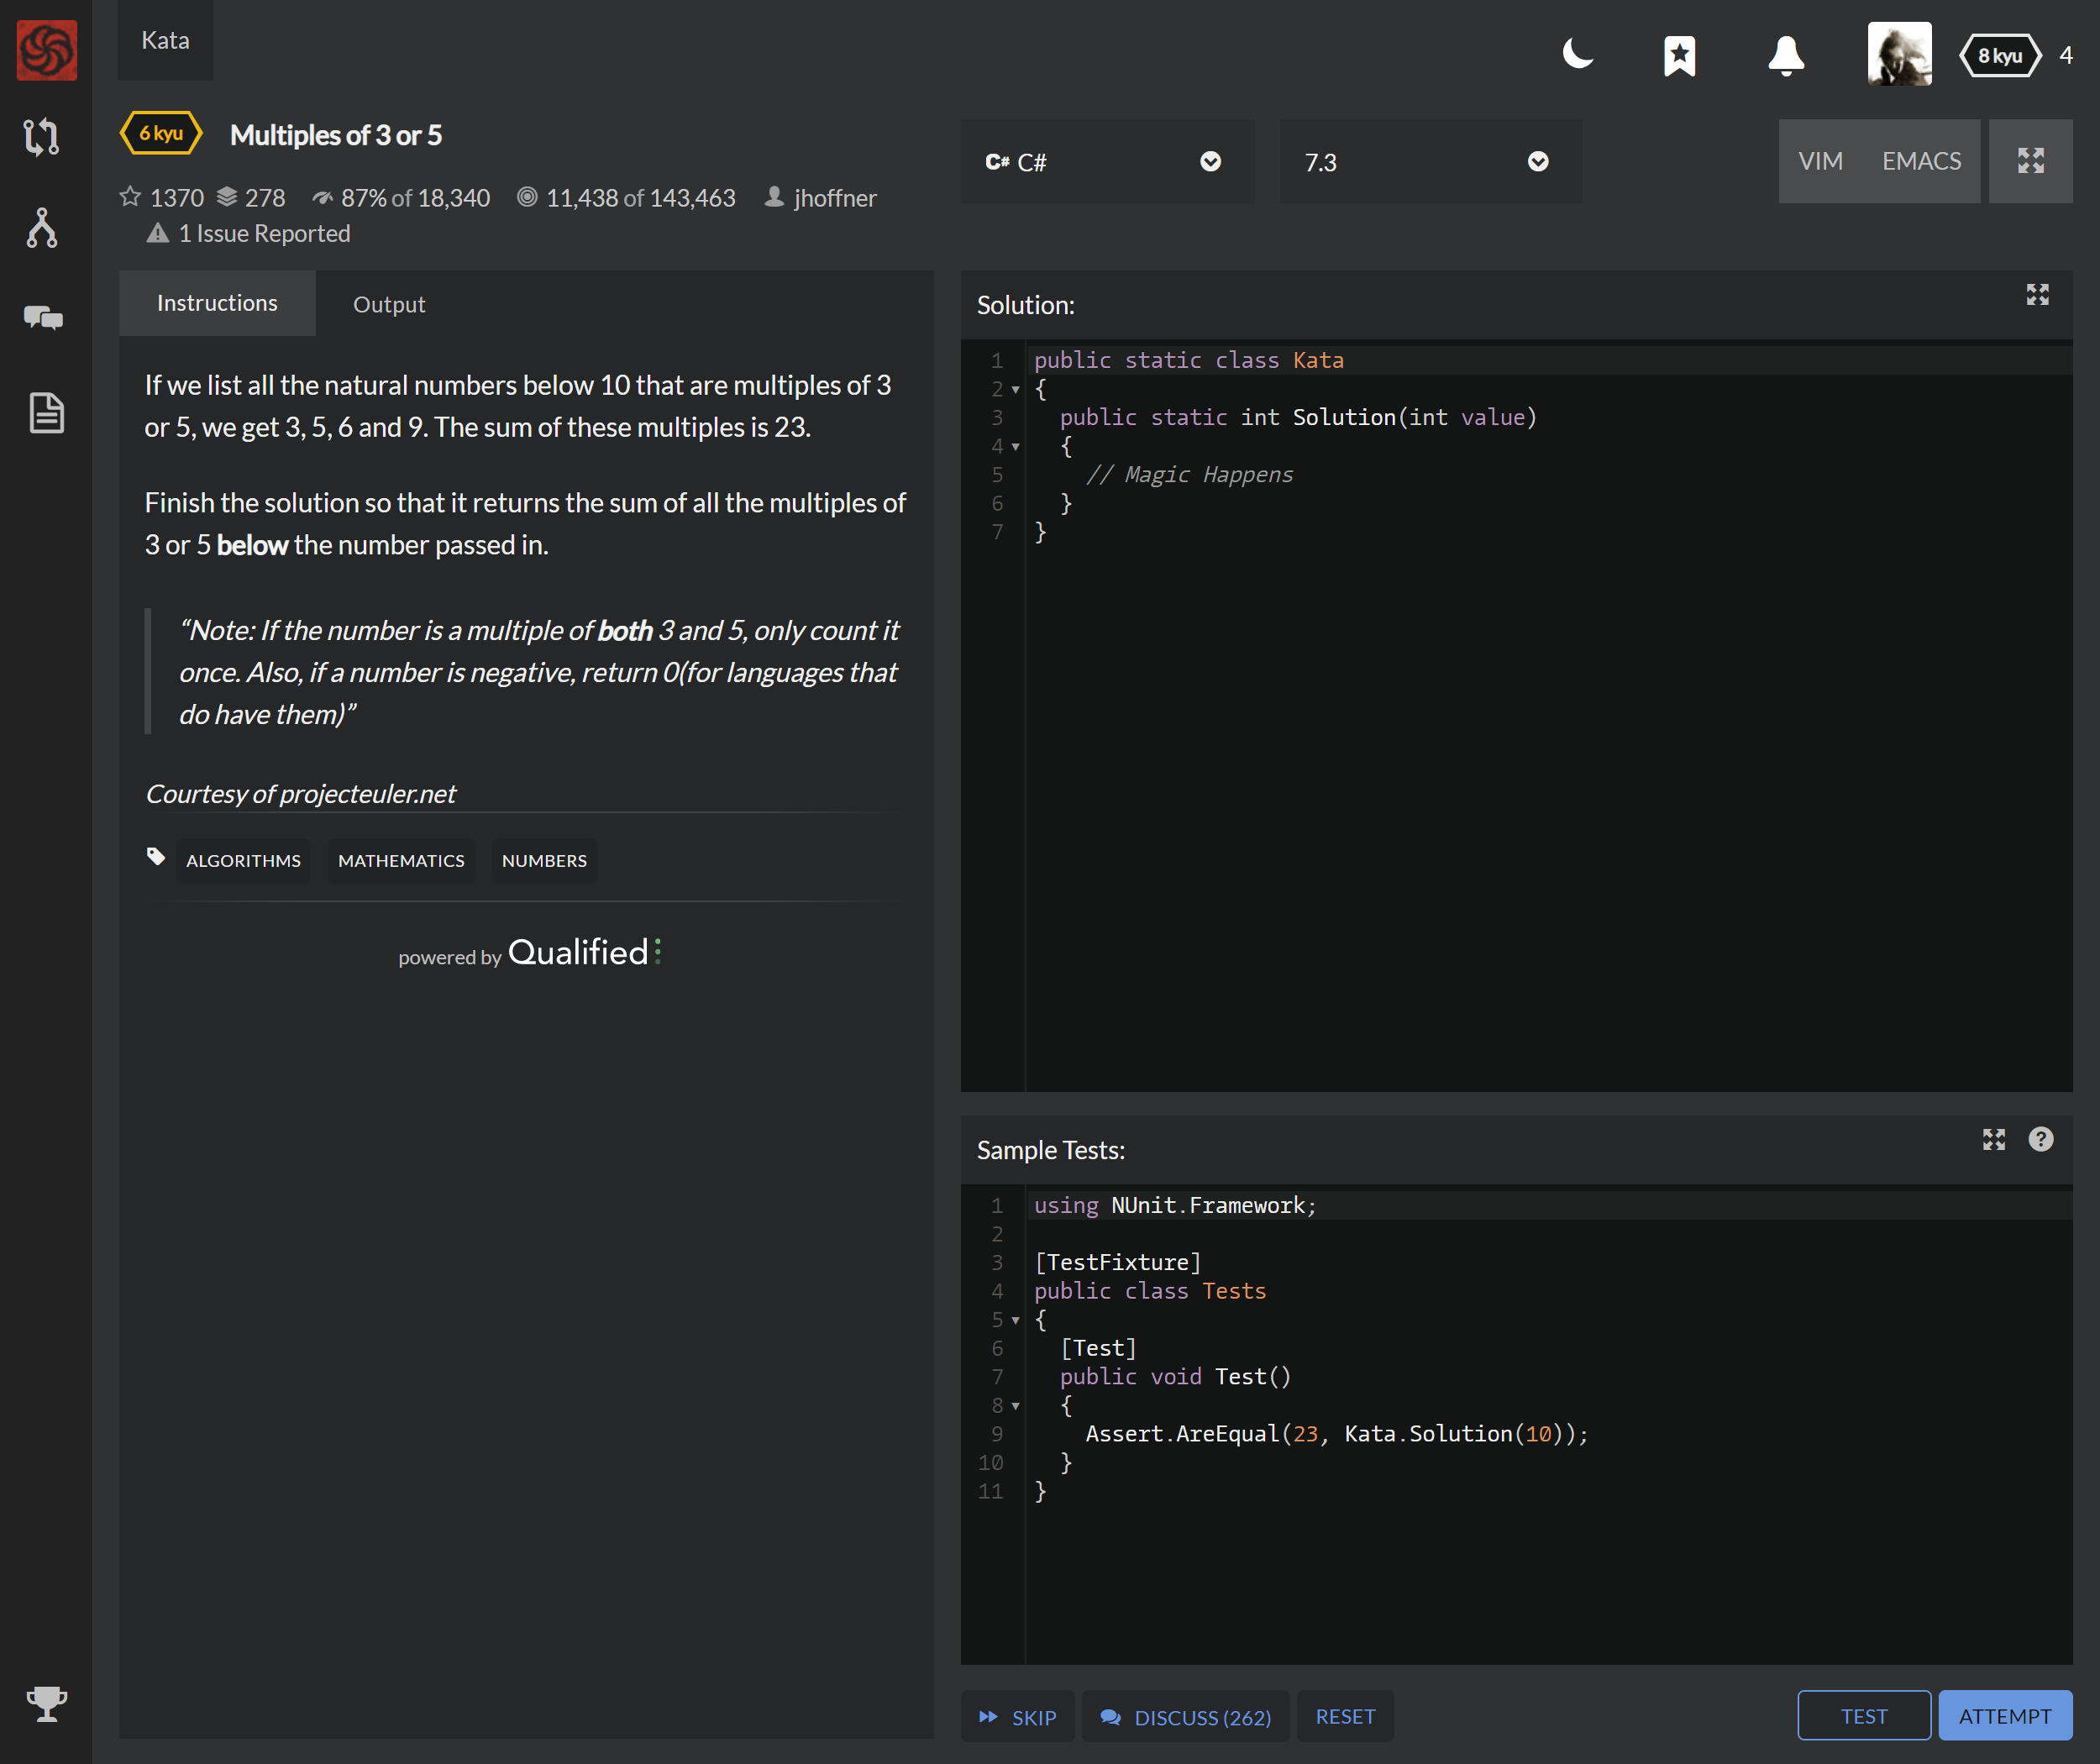
\includegraphics[width=0.95\textwidth]{images/codewars_editor.png}
    \caption{A CodeWars kódszerkesztő felülete.}
    \label{fig:codewars_editor}
\end{figure}

\Aref{fig:codewars_homepage} ábrán látható a CodeWars kódszerkesztő felülete, ami a CodeMirror nevű JavaScript szövegszerkesztő komponenst használja. Itt egy ablakban látjuk a feladat leírását, a korábbi megoldásainkat, és magát a kódot. Állíthatunk világos és sötét mód között, és eltüntethetjük az alkalmazás nem kívánt részeit, hogy a szerkesztőfelületünk nagyobb legyen, és akár rögtön a szerkesztőben válthatunk programozási nyelvet is, és az ahhoz tartozó fordító verziót.

Ezenkívül a Mesterhez hasonlóan az alkalmazás képes szerveroldalon lefuttatni és letesztelni a kódunkat, így az egészhez csak egy böngészőre van szükségünk hiszen semmit sem kell lokálisan a saját gépünkön végezni.

Korlátozás a weboldalban az, hogy egyetlen nyelven sem érhető el a kódkiegészítés funkció, így a valódi fejlesztőkörnyezetekhez képest vakon kell kódot írnunk, és gyakran olvasni kell a dokumentációt, hogy milyen lehetőségeink vannak egy nem ismert osztálynál vagy metódusnál.

A tesztek lefuttatása esetén a futtatás eredményét, a tesztek kimenetét, esetleges fordítási hibákat, illetve a futási időt látjuk szerkesztőnkben.

A kódunk megírása után két lehetőségünk van. \Aref{fig:codewars_editor} ábrán látható egy \emph{Sample Tests} (minta tesztesetek) ablak, ahol a feladat készítője szolgáltatott nekünk egy minta tesztet. Ezt akár szerkeszthetjük vagy adhatjuk hozzá saját teszteseteket, mintha a tesztvezérelt fejlesztés elve szerint oldanánk meg a feladatot. A \emph{Test} gomb a minta tesztesetek ablakban található teszteket fogja lefuttatni. Viszont a \emph{Attempt} (beadás) gomb már a feladat készítője által írt, számunkra rejtett teszteseteket futtatja le, majd ha minden teszt sikeres akkor késznek tekinti a megoldásunkat.

\SubSection{LeetCode}

A LeetCode egy online, programozási problémákat és feladatok kínáló weboldal. Az oldal fő témája az állásinterjúk programozási és algoritmizáló részére való felkészítés. \cite{leetcode} Nagyban hasonlít az előzőleg már említett CodeWars-hoz, de magáról az oldal hátteréről vagy működéséről kevés információ érhető el.

\begin{figure}[h]
    \centering
    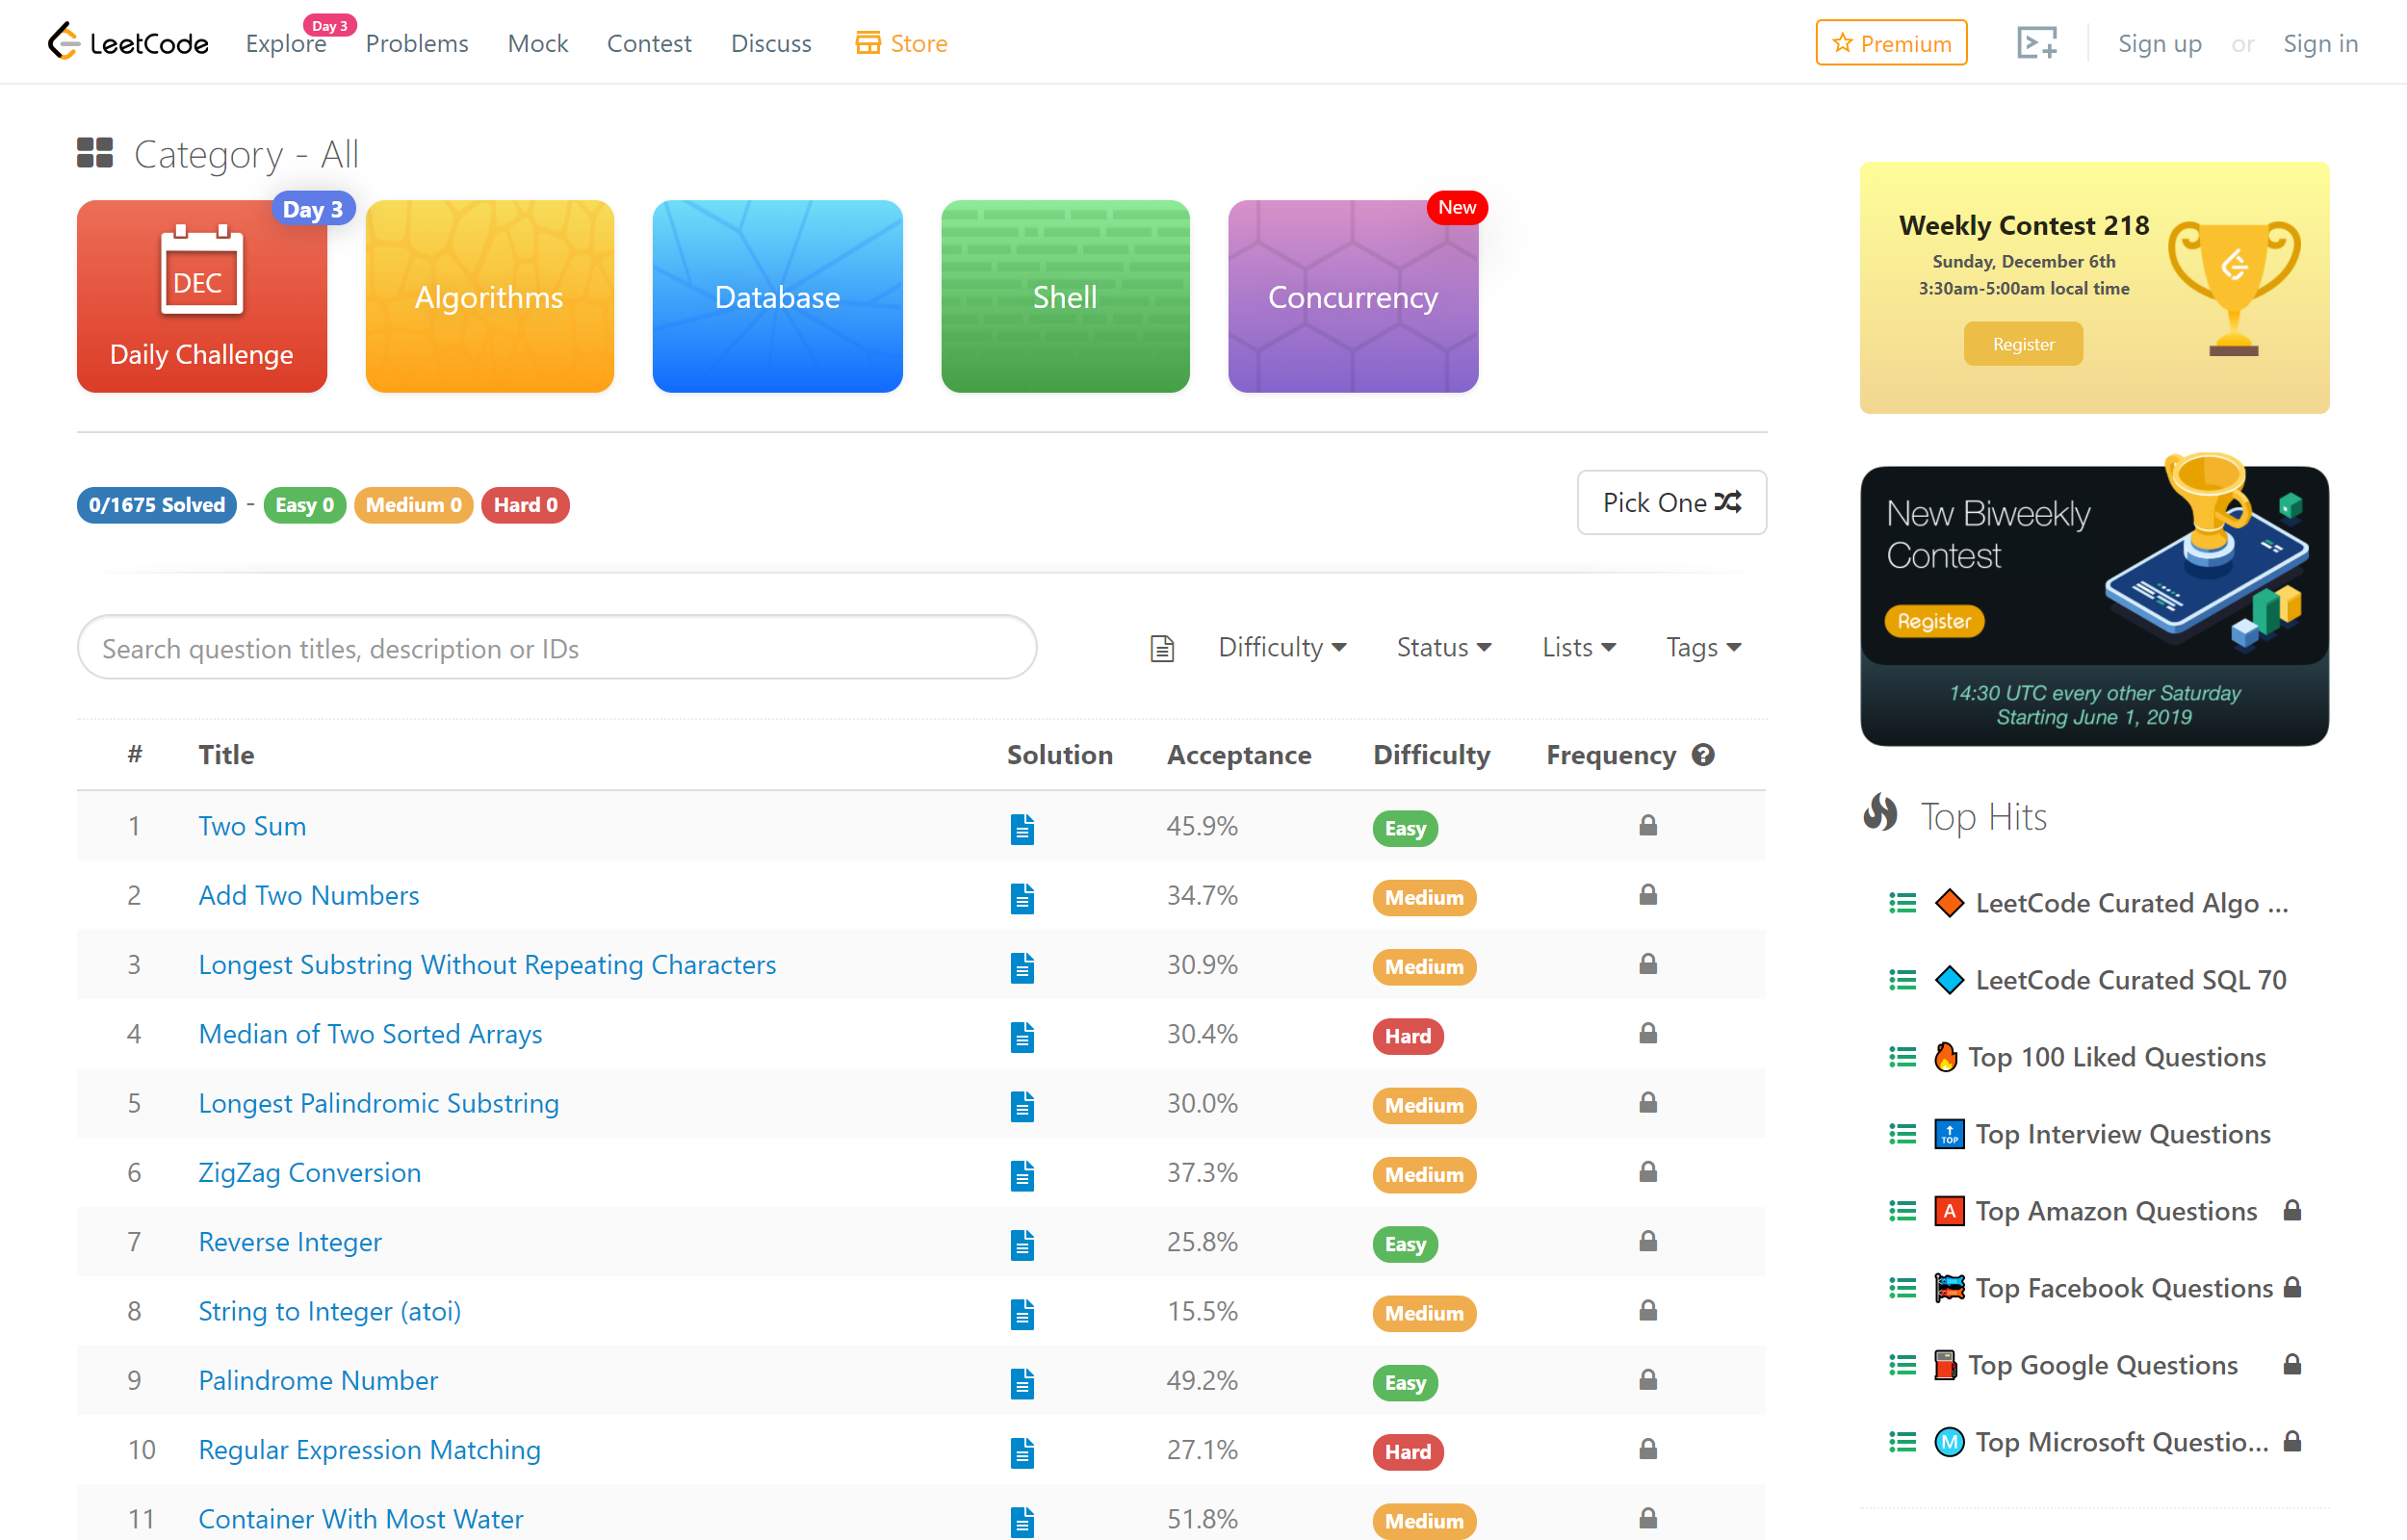
\includegraphics[width=0.95\textwidth]{images/leetcode_problems.png}
    \caption{A LeetCode főoldala, és a megoldható feladatok kilistázva.}
    \label{fig:leetcode_problems}
\end{figure}

Az oldalon több mint 1600 feladat található meg, amiket 15 különböző nyelven oldhatunk meg. Több kategória is létezik az oldalon, a legnépszerűbb Facebook, Amazon, Google és Microsoft interjú feladatokhoz csak havi vagy éves előfizetés után férhetünk hozzá. Ezenkívül vannak napi és havi kihívások is az oldalon. Részben ez is gamifikált rendszer, de nem erre viszi el a hangsúlyt, mint a CodeWars.

A feladatok csoportosítva vannak nehézség és témakör szerint, illetve láthatjuk minden feladatnak a megoldási arányait is.

Rögtön elérjük az összes ingyenes feladatot, illetve azok megoldásait is. Általában többféle megoldás is fel van töltve, ezek főként Java nyelven vannak kidolgozva, de van ahol több nyelven is elérjük a példamegoldásokat.

\begin{figure}[h]
    \centering
    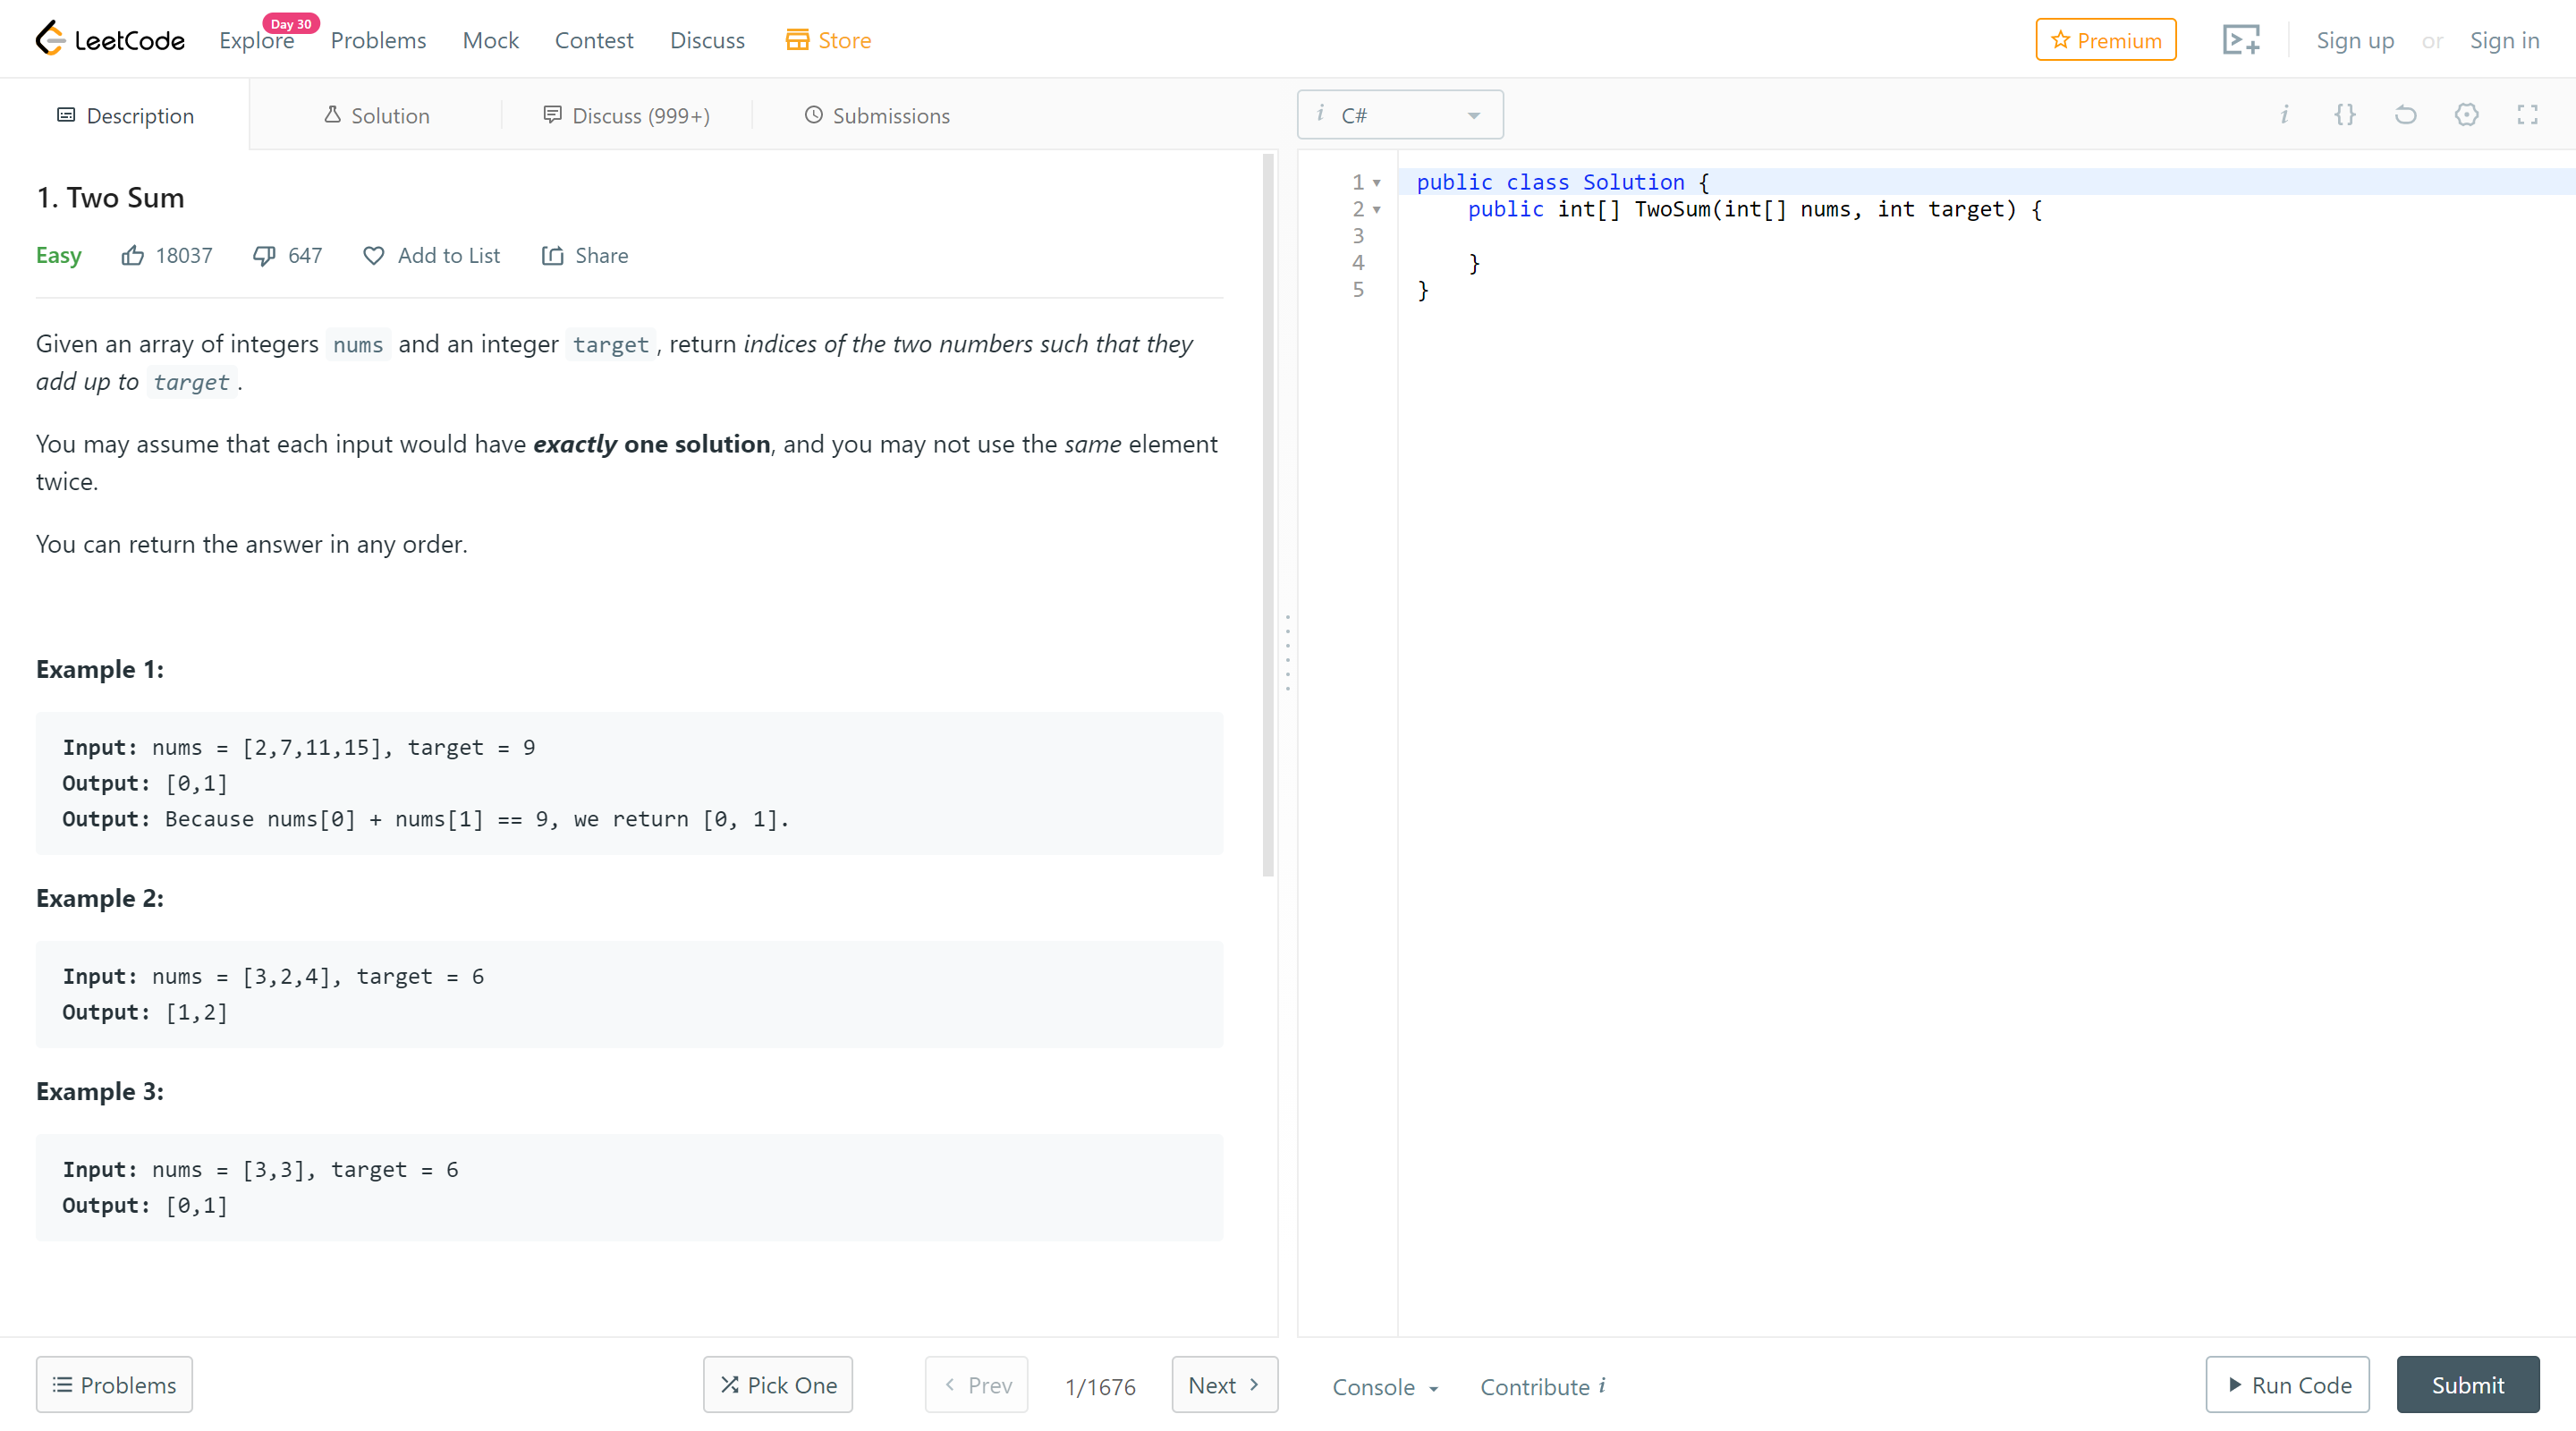
\includegraphics[width=0.95\textwidth]{images/leetcode_editor.png}
    \caption{A LeetCode kódszerkesztő felülete.}
    \label{fig:leetcode_editor}
\end{figure}

A teljesen online kódszerkesztő és futtató felület nagyon egyszerű és letisztult, rögtön láthatjuk a feladatleírást, ezenkívül külön menüpontban elérhetőek a mintamegoldások, hozzászólás szekció és a korábbi megoldásaink. Szokásosan jobb oldalt kapott helyet a kódszerkesztő komponens, ami itt is a CodeMirror nevű JavaScript könyvtárt használja. Itt válthatunk a 15 különböző nyelv között, persze a legnépszerűbb nyelvek elérhetők mint például a C\#, Java, JavaScript vagy a Python 2 és 3. A kódkiegészítés prémium funkcióként elérhető ezeknél a nyelveknél, viszont ezekre az előbb is említett fizetős csomagra kell váltanunk. C\#-nál a fizetős csomagban sem érhető el sajnos a kódkiegészítés.

Ez az oldal is a tesztvezérelt oktatás elvén működik és egységtesztelő keretrendszert használ a megoldásaink kiértékelésére. Itt nem a standard be- és kimeneteket kell használnunk, hanem a paraméterekkel és kimeneti értékkel kommunikálunk.

Látható még egy minta teszteset, amit az előző oldalakhoz hasonlóan módosíthatunk és akár bővíthetjük is, és a program lefutása után a futási üzenetet is megkapjuk. Prémium funkcióként elérhető a hibakereső (\emph{debugger}) felület is.

\SubSection{Exercism}

Az Exercism egy online, ingyenes, nyílt forráskódú programozási platform, ami kódolási gyakorlást és mentorálást igér mindenkinek. Az oldalon több mint 3000 feladatot oldhatunk meg 52 különböző nyelven. \cite{exercism}

A legnépszerűbb nyelvek mind támogatottak, mint például a C\#, Java, JavaScript, Python, de ezenkívül akár x86-64 assembly-ben vagy Prolog-ban is oldhatunk meg feladatokat.

\begin{figure}[h]
    \centering
    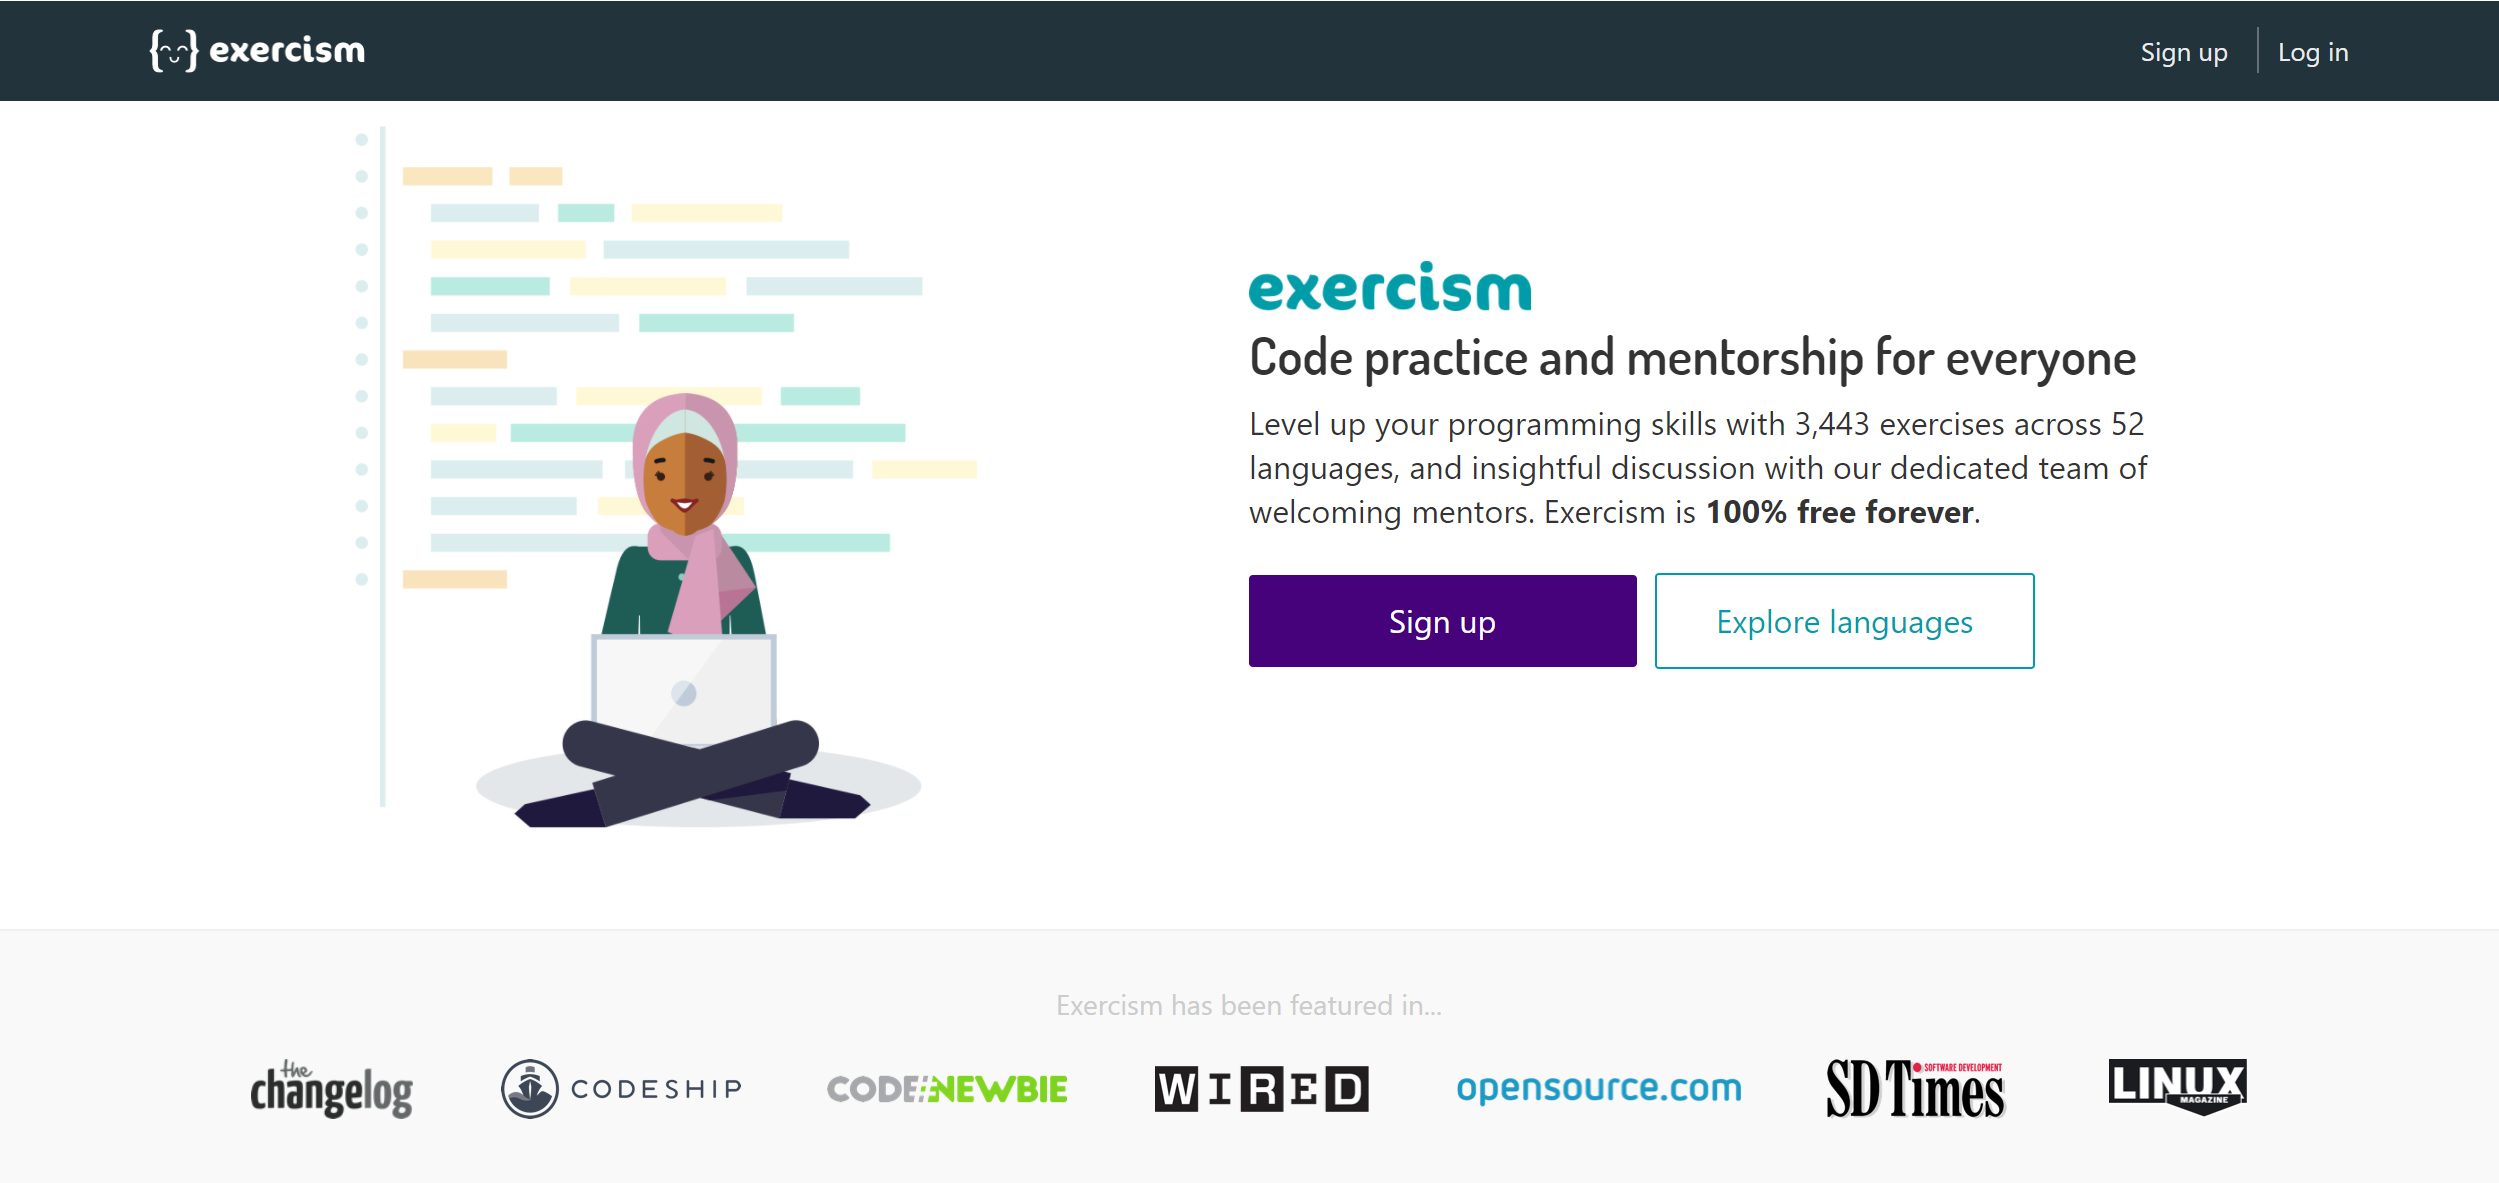
\includegraphics[width=0.95\textwidth]{images/exercism_homepage.png}
    \caption{Az Exercism főoldala.}
    \label{fig:exercism_homepage}
\end{figure}

Ez az oldal abban tér el a többitől, hogy nem kínálnak online kódszerkesztési lehetőséget, hanem valós életbeli projekteket szimulálva kínálnak egy saját fejlesztésű parancssoros klienst, amivel a feladatokat lokálisan letöltve tudjuk megoldani és ellenőrizni a tesztekkel. Ez arra is biztatja a tanulókat, hogy megtanuljanak egy kódszerkesztőt vagy integrált fejlesztői környezetet és magát a parancssort magabiztosan használni, ezen tudásukat később pedig újrahasznosíthatják valós életbeli projekteknél.

A kliens lehetőséget nyújt arra, hogy a megoldásaikat feltöltsék az Exercism rendszerébe ezáltal a mentorok át tudják tekinteni és értékelni. A mentorok önkéntesek és teljesen ingyenesen segítenek mindenkinek.

A feladatok programozási nyelvek szerint kurzusokba vannak csoportosítva, és minden kurzus 40-100 feladatot tartalmaz. A kurzusokon belül könnyű--közepes--nehéz nehézségi szint alapján vannak csoportosítva a feladatok, illetve konkrét programozási fogalmak szerint is fel vannak címkézve azok (például: tömbök, osztályok, string-ek).

Egy feladatot megnyitva láthatjuk azon leírását, ami itt is szintén Markdown formátumban van megadva, és időnként \LaTeX{} kódot is tartalmaz. Miután a feladatot a parancssoros kliens segítségével letöltjük, megkapjuk azt egy projekt formájában, ami tartalmaz egy kiinduló programkódot az osztály és metódusdefiníciókkal, illetve egy teszteseteket tartalmazó fájlt. A teszteket a programozási nyelv hagyományos módján tudjuk lefuttatni, mivel a tesztesetek minden esetben egy egységtesztelő keretrendszerrel vannak írva. A kurzusok biztatják a felhasználót a tesztvezérelt fejlesztésre, alapértelmezetten az összes feladatnál csak az első teszteset van engedélyezve, a többit a tanulónak kell engedélyezni a fejlesztés során.

A feladat specifikációi egy közös, nyelvfüggetlen metaadatbankban vannak tárolva, és ezen kanonikus adatok alapján adott nyelvi generátor programokkal generálják a programozási nyelvekhez a teszteseteket. \cite{exercism_problem-specifications} \cite{exercism_csharp-generator}

\SubSection{HackerRank}

A HackerRank egy kompetitív programozási kihívásokat, feladatokat kínáló weboldal, amelyen a fejlesztők egymással mérkőzhetnek meg a feladatok megoldásával. Az oldal a szokványos algoritmizáló és interjúztatási feladatokon kívül a számítógép-tudomány több ágáról is biztosít feladatokat, ilyenek többek között a mesterséges intelligencia, funkcionális programozás, adatbázisok-adatstruktúrák és a gépi tanulás. \cite{hackerrank} \cite{hackerrank_faq}

Az oldalon több mint 40 nyelven oldhatnak meg feladatokat a fejlesztők, ezek között elérhető a C++, Python, Java több verziója illetve JavaScript, C\# is. \cite{hackerrank_environment}

A feladatok a témakör vagy programozási nyelv szerinti csoportosításban szerepelnek, ezenbelül szűrhetünk még altémákra és nehézségi szintre is. A Project Euler-féle szöveges, matematikával kapcsolatos programozási feladatok is elérhetőek az oldalon teljesen automatizáltan tesztelhető formában is.

\begin{figure}[h]
    \centering
    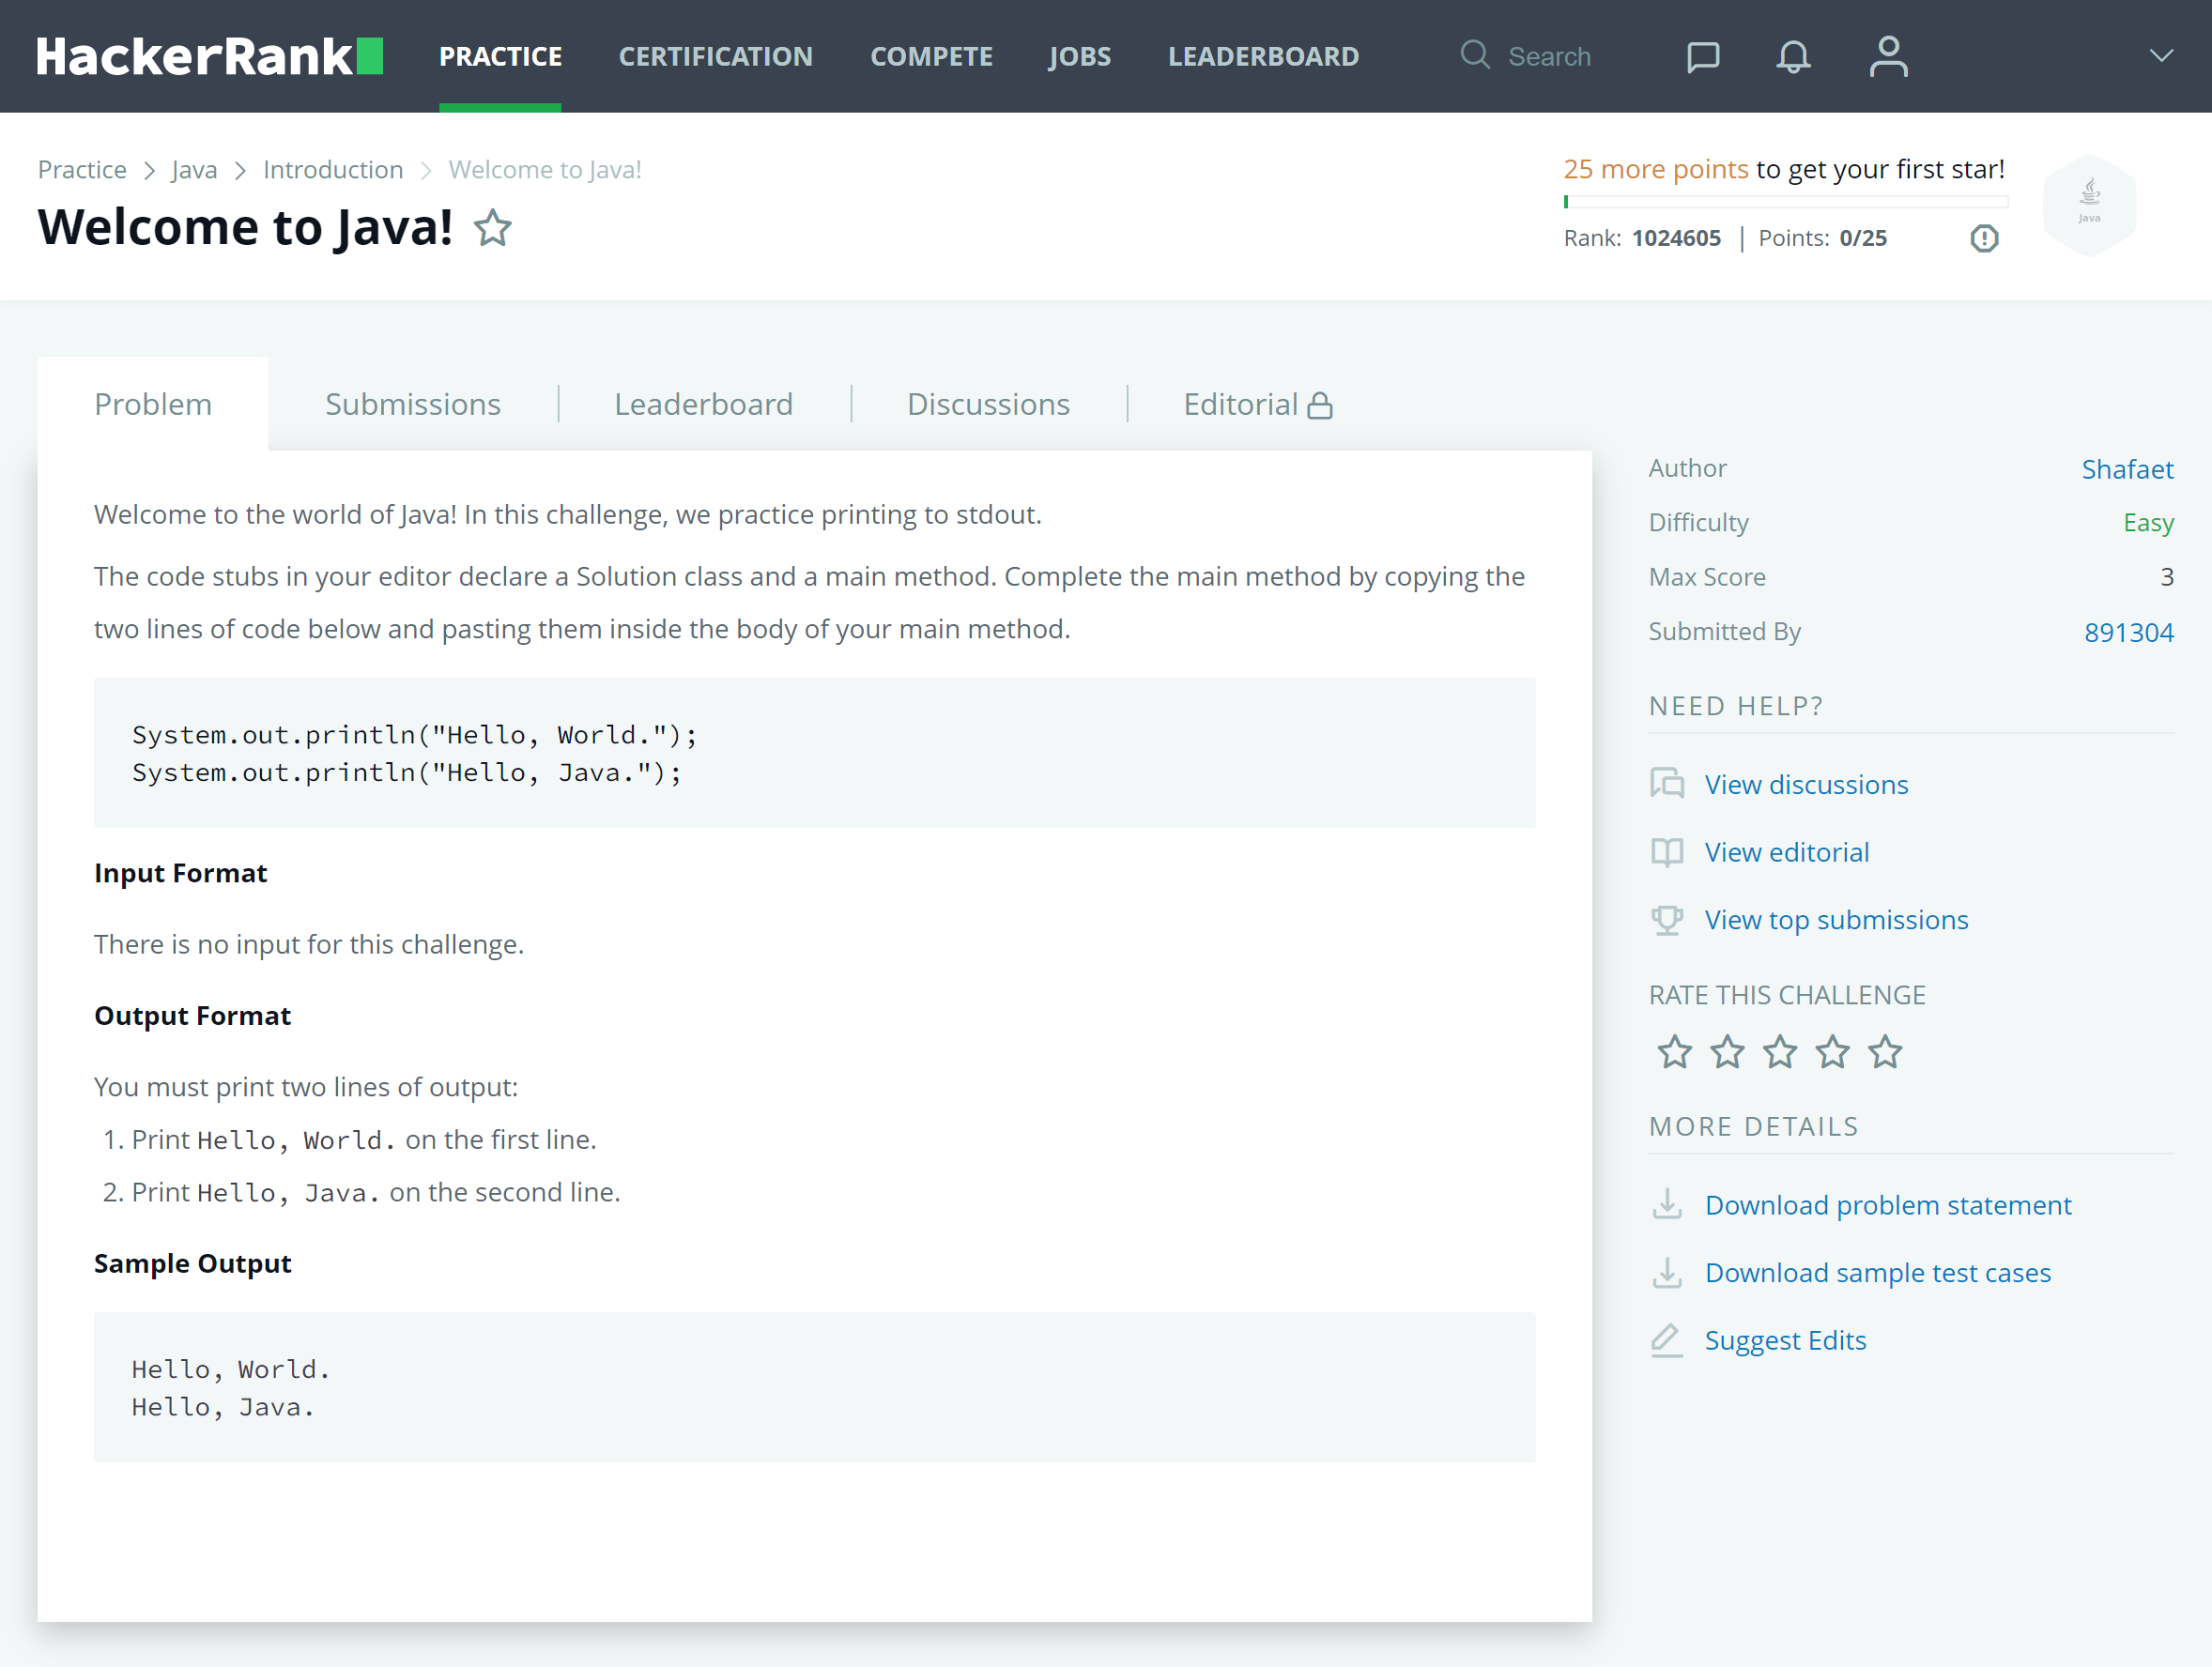
\includegraphics[width=0.95\textwidth]{images/hackerrank_task.png}
    \caption{Egy HackerRank-on található feladat leírása.}
    \label{fig:exercism_task}
\end{figure}

A feladatok leírása Markdown és MathJax segítségével vannak megjelenítve.

A weboldal igaz nem nyílt forráskódú, de a legújabb technológiákat veszi, ilyen például a Monaco kódszerkesztő komponens, amit a Microsoft fejleszt a Visual Studio Code nevű fejlesztőkörnyezethez. Ezáltal elérhető minden nyelvhez az automatikus kódkiegészítés.

\begin{figure}[h]
    \centering
    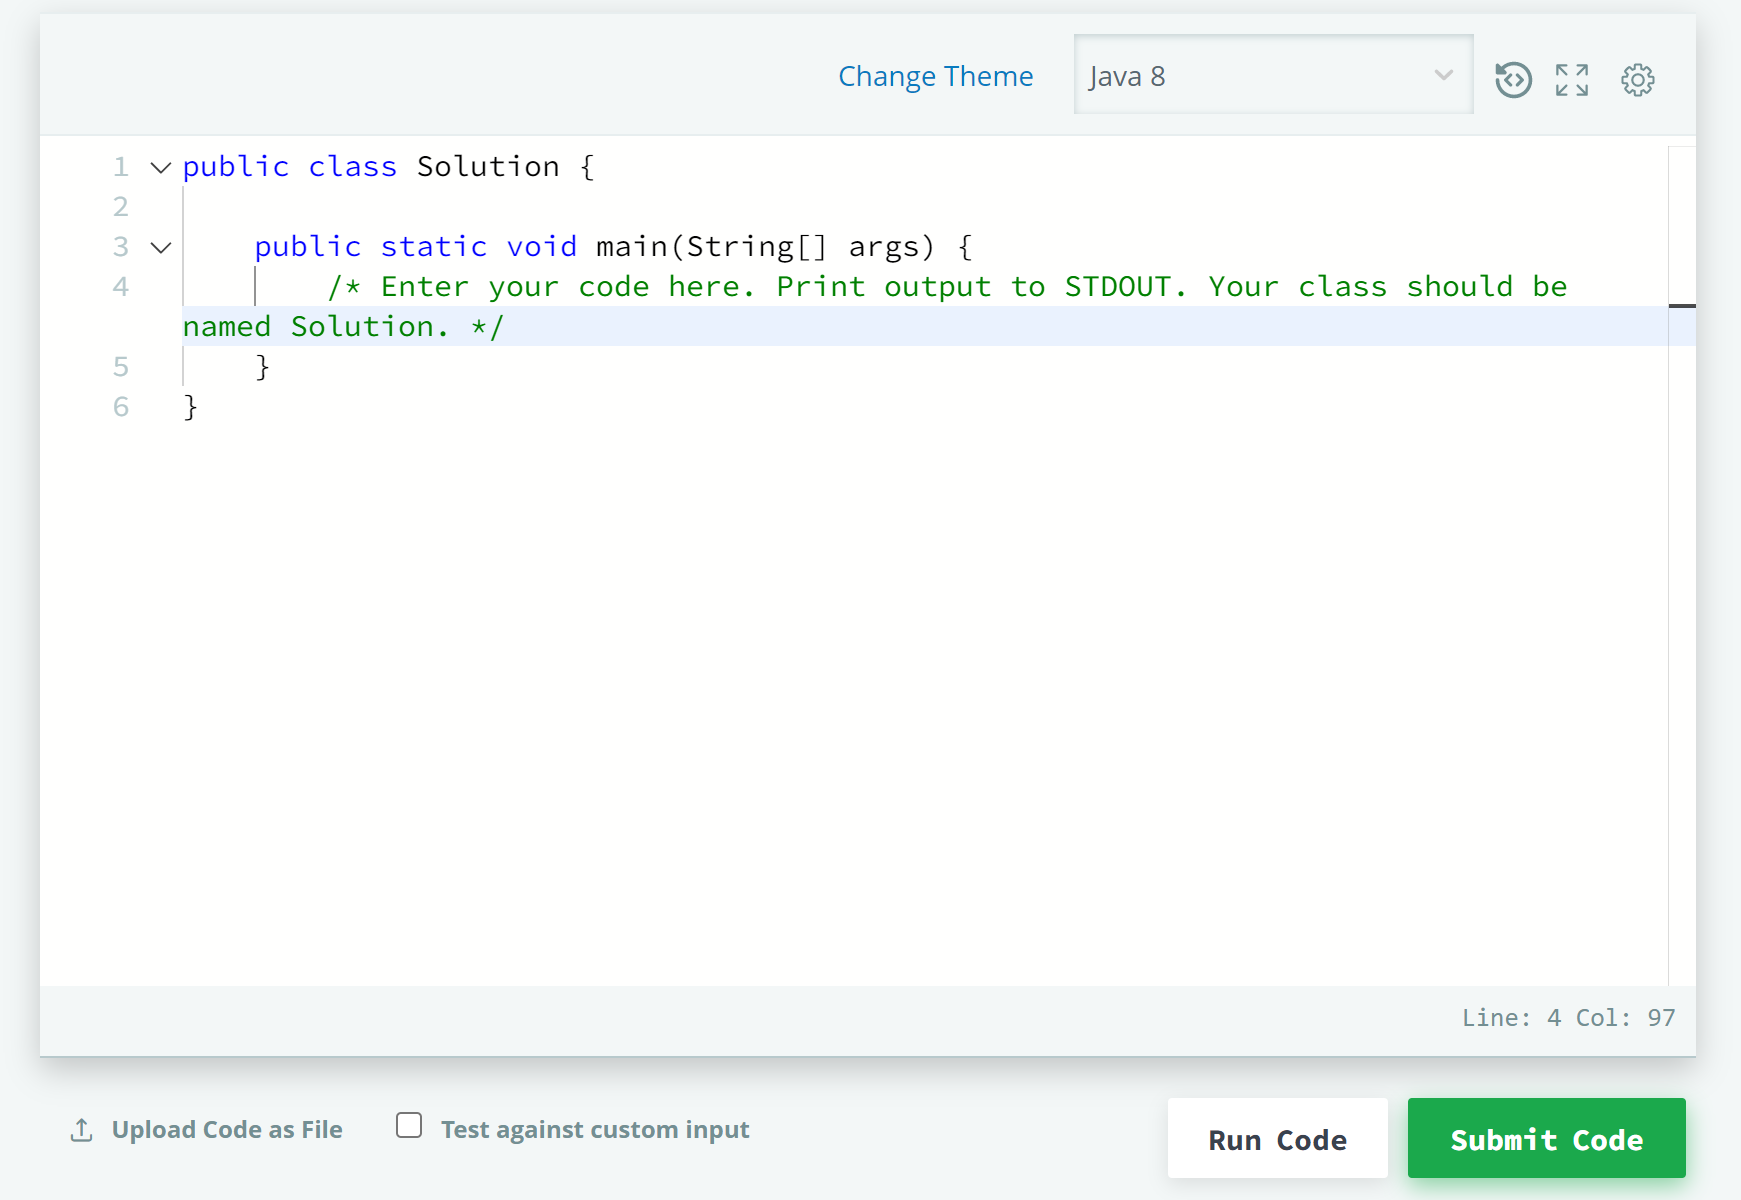
\includegraphics[width=0.95\textwidth]{images/hackerrank_editor.png}
    \caption{A HackerRank kódszerkesztő felülete.}
    \label{fig:hackerrank_editor}
\end{figure}

A kódszerkesztőben elérhető világos, sötét, illetve nagy kontrasztú mód is, ezenkívül átválthatunk teljes képernyős szerkesztési módba is. Sajnos azt nem lehet állítani, hogy a szerkesztő és a feladatleírás ne egymás alatt legyen, hanem egymás mellett mint az előzőleg bemutatott oldalakon.

Ez az alkalmazás is teljesen automatizáltan a böngészőből működik, viszont nem bemeneti argumentumokkal és visszatérési értékekkel kell operálnunk hanem a standard ki- és bemenetet kell használni.

Az oldalon található egy információk szekció ahol szépen le van vezetve, hogy az adott nyelven milyen idő- és memóriakorlát van bevezetve, milyen verziójú fordítót használ a szerver és milyen függvénykönyvtárakat érünk el. C\# esetén Mono 6.4 fordítót használ a rendszer amivel a .NET Framework 4.7.2 funkcióit érjük el, és 3 másodperc időkorlát, 512 MB memóriakorlát van jelen. Függvénykönyvtárak esetén a Newtonsoft által készített JSON könyvtárat és a Microsoft által karbantartott HttpClient és WebClient könyvtárakat érjük el. JavaScript esetén a Node.js 10-es verziójához férünk hozzá, itt egy növelt 10 másodperces időkorlát és szintúgy 512 MB memóriakorlát érhető el. Függvénykönyvtárak esetében pedig a következőkhöz férünk hozzá: bignumber.js, jquery, lodash, underscore, request, axios. A programjaink egy virtualizált 64-bites Ubuntu rendszeren futnak, és minden nagyobb nyelven elérhető a több szálon való futtatás, az időkorlátban ez is figyelembe van véve. \cite{hackerrank_environment}

\SubSection{Összehasonlítás}
% TODO: beautify table
{
    \footnotesize
    \begin{tabularx}{\textwidth}{@{}X|X|X|X|X|X@{}}
                                                                                                                    &
        \textbf{Mester}                                                                                             &
        \textbf{CodeWars}                                                                                           &
        \textbf{LeetCode}                                                                                           &
        \textbf{Exercism}                                                                                           &
        \textbf{HackerRank}{}                                                                                         \\ \hline \endhead
        \textbf{programozási nyelvek száma}                                                                         &
        6                                                                                                           &
        \textgreater{} 50                                                                                           &
        15                                                                                                          &
        52                                                                                                          &
        \textgreater{} 40                                                                                             \\ \hline
        \textbf{feladatok száma}                                                                                    &
        $\sim$ 2000                                                                                                 &
        \textgreater{} 9000                                                                                         &
        \textgreater{} 1600                                                                                         &
        \textgreater{} 3000                                                                                         &
        nincs megadva                                                                                                 \\ \hline
        \textbf{feladatok csoportosítása}                                                                           &
        szint és téma szerinti                                                                                      &
        nehézség és témakör szerinti                                                                                &
        nehézség és témakör szerinti                                                                                &
        nyelv, nehézség és programozási fogalmak alapján                                                            &
        témakör, nyelv és nehézségi szint, altémák szerinti                                                           \\ \hline
        \textbf{feladatok elérhetősége}                                                                             &
        összes                                                                                                      &
        összes                                                                                                      &
        összes ingyenes                                                                                             &
        összes                                                                                                      &
        összes                                                                                                        \\ \hline
        \textbf{feladatok leírása}                                                                                  &
        PDF                                                                                                         &
        Markdown + \LaTeX{}                                                                                         &
        HTML                                                                                                        &
        Markdown + \LaTeX{}                                                                                         &
        Markdown + \LaTeX{}                                                                                           \\ \hline
        \textbf{minta}                                                                                              &
        2 nyelven kidolgozott mintafeladat minden témához, minden feladathoz 2 db példa ki- és bemenet              &
        minta\-feladatok nincsenek; mintatesztek elérhetőek minden feladatnál                                       &
        minta\-feladatok nincsenek; mintamegoldás mindenhol elérhető, főként Java nyelven és sokszor fizetősen      &
        nincs                                                                                                       &
        minta be- és kimenet minden feladatnál meg van adva, nincs mintafeladat                                       \\ \hline
        \textbf{limitek}                                                                                            &
        feladatonként idő- és memórialimit                                                                          &
        nyelvenként egységes időlimit, memórialimitet nem ad meg az oldal                                           &
        nem ad meg az oldal limiteket, feltételezhetően van időlimit                                                &
        nincs                                                                                                       &
        nyelvenként idő- és memórialimit                                                                              \\ \hline
        \textbf{korlátozások}                                                                                       &
        limitált programfuttatás feladatonként, nincs online szerkesztő                                             &
        nincs kódkiegészítés, mások megoldásait csak a saját, jó megoldásunk beadása után látjuk                    &
        kódkiegészítés fizetős funkcióként elérhető                                                                 &
        nincs online kódszerkesztő és tesztfuttató környezet                                                        &
        nincs                                                                                                         \\ \hline
        \textbf{pontozás}                                                                                           &
        0-100, feladatonként eltérő                                                                                 &
        nincs                                                                                                       &
        nincs                                                                                                       &
        nincs                                                                                                       &
        van, feladatonként dinamikusan számolt                                                                        \\ \hline
        \textbf{függvény\-könyvtárak}                                                                               &
        csak standard, platformspecifikusok letiltva                                                                &
        nincs meghatározva                                                                                          &
        nincs meghatározva                                                                                          &
        bármi használható                                                                                           &
        nyelvenként eltérő                                                                                            \\ \hline
        \textbf{ellenőrzés típusa}                                                                                  &
        STDIN, STDOUT                                                                                               &
        metódus paraméterek és visszatérési érték                                                                   &
        metódus paraméterek és visszatérési érték                                                                   &
        metódus paraméterek és visszatérési érték                                                                   &
        STDIN, STDOUT                                                                                                 \\ \hline
        \textbf{gamifikáció}                                                                                        &
        nem                                                                                                         &
        igen                                                                                                        &
        részben                                                                                                     &
        nem                                                                                                         &
        részben, kompetitív                                                                                           \\ \hline
        \textbf{megoldások}                                                                                         &
        mások megoldása nem látható, a korábbi megoldásainkat látjuk, az adatokkal együtt                           &
        mások megoldásai a sajátunk beadása után látható                                                            &
        mások megoldásait láthatjuk, a korábbi megoldásaink is megtekinthetőek, a mintamegoldások sokszor fizetősek &
        mások megoldásait láthatjuk, saját megoldásunk is megtekinthető                                             &
        saját és mások megoldásai is elérhetőek                                                                       \\ \hline
        \textbf{kódszerkesztő}                                                                                      &
        nincs                                                                                                       &
        van, CodeMirror                                                                                             &
        van, CodeMirror                                                                                             &
        lokális                                                                                                     &
        van, Monaco                                                                                                   \\ \hline
        \textbf{tesztfuttató}                                                                                       &
        van                                                                                                         &
        van                                                                                                         &
        van                                                                                                         &
        van, de lokálisan                                                                                           &
        van                                                                                                           \\ \hline
        \textbf{eredmények}                                                                                         &
        a futási időt, a hibakódot és a pontszámot jelzi ki                                                         &
        futási idő, hibaüzenet és kimenet jelzése                                                                   &
        hibaüzenet jelzése, és prémium funkcióként debugger is elérhető                                             &
        lokálisan minden látszódik                                                                                  &
        futási üzenet, hibaüzenetek kijelzése, futási idő nem látszódik
    \end{tabularx}
}

\Section{Technológia}

% Mivel jellemzően kutatásról vagy szoftverfejlesztésről van szó, ezért annak a jellemző elemeit, technikai részleteit itt kell bemutatni.
% Ez tehát egy módszeres bevezetés ahhoz, hogy ha valaki nem jártas a témakörben, akkor tudja, hogy a dolgozat milyen aktuálisan elérhető eredményeket, eszközöket használt fel.

\SubSection{Elmélet}

\subsubsection{Tiszta architektúra}

\cite{martin_2017_clean-architecture} \cite{martin_2012_the-clean-architecture}

\begin{figure}[h]
    \centering
    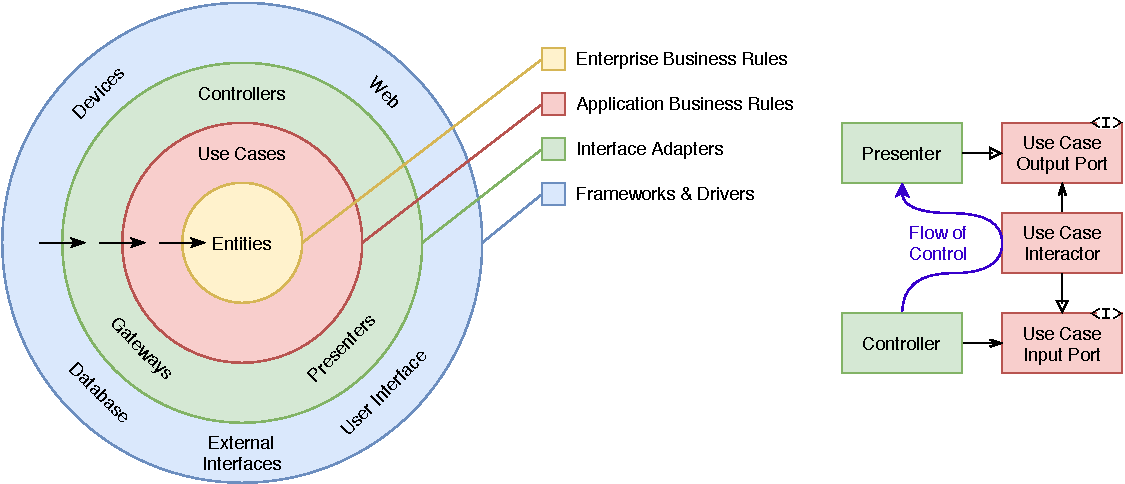
\includegraphics[width=0.95\textwidth]{images/clean-architecture_unclebob.pdf}
    \caption{A Robert C. Martin által készített Tiszta architektúra diagram.}
    \label{fig:clean-architecture_unclebob}
\end{figure}

\begin{figure}[h]
    \centering
    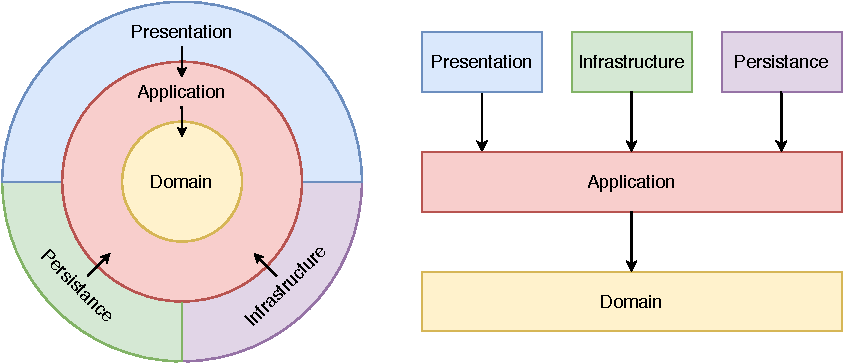
\includegraphics[width=0.95\textwidth]{images/clean-architecture_simplified.pdf}
    \caption{A Jason Taylor által leegyszerűsített Tiszta architektúra diagram.}
    \label{fig:clean-architecture_simplified}
\end{figure}

\subsubsection{Parancs--lekérdezés felelősség elkülönítése}

\subsubsection{Közvetítő (mediator) programtervezési minta}

\begin{figure}[h]
    \centering
    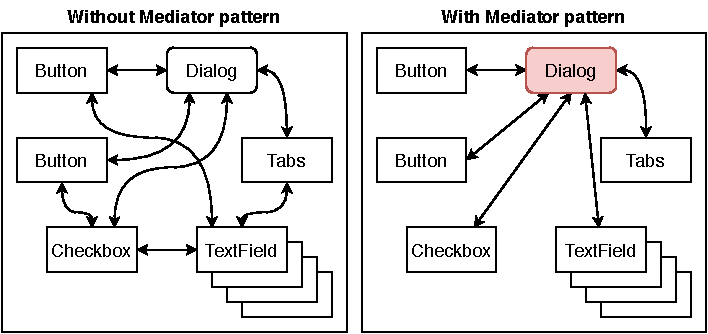
\includegraphics[width=0.95\textwidth]{images/mediator_pattern.pdf}
    \caption{A Mediator pattern diagram.}
    \label{fig:mediator_pattern}
\end{figure}

\SubSection{Kliens}

\subsubsection{Angular}

\subsubsection{Bootstrap}

\subsubsection{TypeScript}

\subsubsection{Sass}

\subsubsection{Monaco Editor}

\SubSection{Szerver}

\subsubsection{ASP.NET Core}

\subsubsection{Entity Framework Core}

\subsubsection{MediatR}

\subsubsection{Roslyn}

\subsubsection{xUnit.net}

\Section{Követelmény specifikáció}

% Külön szakaszban érdemes részletesen kitérni az elkészítendő alkalmazással kapcsolatos követelményekre.
% Ehhez tartozhatnak forgatókönyvek (\textit{scenario}-k).
% A szemléletesség kedvéért lehet hozzájuk képernyőkép vázlatokat is készíteni, vagy a használati eseteket más módon szemléltetni.

\Chapter{Tervezés}

Itt kezdődik a dolgozat lényegi része, úgy értve, hogy a saját munka bemutatása.
Jellemzően ebben szerepelni szoktak blokkdiagramok, a program struktúrájával foglalkozó leírások.
Ehhez célszerű UML ábrákat (például osztály- és szekvenciadiagramokat) használni.

Amennyiben a dolgozat inkább kutatás jellegű, úgy itt lehet konkretizálni a kutatási módszertant, a kutatás tervezett lépéseit, az indoklást, hogy mit, miért és miért pont úgy érdemes csinálni, ahogyan az a későbbiekben majd részletezésre kerül.

Ebben a fejezetben az implementáció nem kell, hogy túl nagy szerepet kapjon.
Ez még csak a tervezési fázis.
(Nyilván ha olyan a téma, hogy magának az implementációnak a módjával foglalkozik, adott formális nyelvet mutat be, úgy a kódpéldákat már innen sem lehet kihagyni.)

\Section{Táblázatok}

Táblázatokhoz a \texttt{table} környezetet ajánlott használni.
Erre egy minta \aref{tab:minta}. táblázat.
A hivatkozáshoz az egyedi \texttt{label} értéke konvenció szerint \texttt{tab:} prefixszel kezdődik.

\begin{table}[h]
\centering
\caption{Minta táblázat. A táblázat felirata a táblázat felett kell legyen!}
\label{tab:minta}
\begin{tabular}{l|c|c|}
a & b & c \\
\hline
1 & 2 & 3 \\
4 & 5 & 6 \\
\hline
\end{tabular}
\end{table}

\Section{Ábrák}

Ábrákat a \texttt{figure} környezettel lehet használni.
A használatára egy példa \aref{fig:cimer}. ábrán látható.
Az \texttt{includegraphics} parancsba 
Az ábrák felirata az ábra alatt kell legyen.
Az ábrák hivatkozásához használt nevet konvenció szerint \texttt{fig:}-el célszerű kezdeni.

\begin{figure}[h]
\centering

\includegraphics[scale=0.3]{images/me_logo.png}
\caption{A Miskolci Egyetem címere.}
\label{fig:cimer}
\end{figure}

\Section{További környezetek}

A matematikai témájú dolgozatokban szükség lehet tételek és bizonyításaik megadására.
Ehhez szintén vannak készen elérhető környezetek.

\begin{definition}
Ez egy definíció
\end{definition}

\begin{lemma}
Ez egy lemma
\end{lemma}

\begin{theorem}
Ez egy tétel
\end{theorem}

\begin{proof}
Ez egy bizonyítás
\end{proof}

\begin{corollary}
Ez egy tétel
\end{corollary}

\begin{remark}
Ez egy megjegyzés
\end{remark}

\begin{example}
Ez egy példa
\end{example}

\Chapter{Megvalósítás}

Ez a fejezet mutatja be a megvalósítás lépéseit.
Itt lehet az esetlegesen előforduló technikai nehézségeket említeni.
Be lehet már mutatni a program elkészült részeit.

Meg lehet mutatni az elkészített programkód érdekesebb részeit.
(Az érdekesebb részek bemutatására kellene szorítkozni.
Többségében a szöveges leírásnak kellene benne lennie.
Abból lehet kiindulni, hogy a forráskód a dolgozathoz elérhető, azt nem kell magába a dolgozatba bemásolni, elegendő csak behivatkozni.)

A dolgozatban szereplő forráskódrészletekhez külön vannak programnyelvenként stílusok.
Python esetében például így néz ki egy formázott kódrészlet.
\begin{python}
import sys

if __name__ == '__main__':
    pass
\end{python}

A stílusfájlok a \texttt{styles} jegyzékben találhatók.
A stílusok között szerepel még C++, Java és Rust stílusfájl.
Ezek használatához a \texttt{dolgozat.tex} fájl elején \texttt{usepackage} paranccsal hozzá kell adni a stílust, majd a stílusfájl nevével megegyező környezetet lehet használni.
További példaként C++ forráskód esetében ez így szerepel.
\begin{cpp}
#include <iostream>

class Sample : public Object
{
    // An empty class definition
}
\end{cpp}
Stílusfájlokból elegendő csak annyit meghagyni, amennyire a dolgozatban szükség van.
Más, C szintaktikájú nyelvekhez (mint például a JavaScript és C\#) a Java vagy C++ stílusfájlok átszerkesztésére van szükség.
(Elegendő lehet csak a fájlnevet átírni, és a fájlban a környezet nevét.)

Nyers adatok, parancssori kimenetek megjelenítéséhez a \texttt{verbatim} környezetet lehet használni.
\begin{verbatim}
$ some commands with arguments
1 2 3 4 5
$ _
\end{verbatim}

A kutatás jellegű témáknál ez a fejezet gyakorlatilag kimaradhat.
Helyette inkább a fő vizsgálati módszerek, kutatási irányok kaphatnak külön-külön fejezeteket.

\Chapter{Tesztelés}

A fejezetben be kell mutatni, hogy az elkészült alkalmazás hogyan használható.
(Az, hogy hogyan kell, hogy működjön, és hogy hogy lett elkészítve, az előző fejezetekben már megtörtént.)

Jellemzően az alábbi dolgok kerülhetnek ide.
\begin{itemize}
\item Tesztfuttatások. Le lehet írni a futási időket, memória és tárigényt.
\item Felhasználói kézikönyv jellegű leírás. Kifejezetten a végfelhasználó szempontjából lehet azt bemutatni, hogy mit hogy lehet majd használni.
\item Kutatás kapcsán ide főként táblázatok, görbék és egyéb részletes összesítések kerülhetnek.
\end{itemize}

\Chapter{Összefoglalás}

Hasonló szerepe van, mint a bevezetésnek.
Itt már múltidőben lehet beszélni.
A szerző saját meglátása szerint kell összegezni és értékelni a dolgozat fontosabb eredményeit.
Meg lehet benne említeni, hogy mi az ami jobban, mi az ami kevésbé jobban sikerült a tervezettnél.
El lehet benne mondani, hogy milyen további tervek, fejlesztési lehetőségek vannak még a témával kapcsolatban.


\clearpage

\addcontentsline{toc}{chapter}{Irodalomjegyzék}
\bibliographystyle{plain}
\bibliography{dolgozat.bib}

\newpage

\pagestyle{empty}

\noindent \textbf{\Large CD Használati útmutató}

\vskip 1cm

Ennek a címe lehet például \textit{A mellékelt CD tartalma} vagy \textit{Adathordozó használati útmutató} is.

Ez jellemzően csak egy fél-egy oldalas leírás.
Arra szolgál, hogy ha valaki kézhez kapja a szakdolgozathoz tartozó CD-t, akkor tudja, hogy mi hol van rajta.
Jellemzően elég csak felsorolni, hogy milyen jegyzékek vannak, és azokban mi található.
Az elkészített programok telepítéséhez, futtatásához tartozó instrukciók kerülhetnek ide.

A CD lemezre mindenképpen rá kell tenni
\begin{itemize}
\item a dolgozatot egy \texttt{dolgozat.pdf} fájl formájában,
\item a LaTeX forráskódját a dolgozatnak,
\item az elkészített programot, fontosabb futási eredményeket (például ha kép a kimenet),
\item egy útmutatót a CD használatához (ami lehet ez a fejezet külön PDF-be vagy MarkDown fájlként kimentve).
\end{itemize}


\end{document}
